\documentclass[14pt,xcolor=dvipsnames,table,dvipdfmx]{beamer}

\usepackage{slide}
\usepackage{appendixnumberbeamer}

\usepackage{math_macros}

\usepackage{import}
\usepackage{url}
\usepackage{diagbox}
\usepackage{array,colortbl}
\usepackage{hyperref}
% \hypersetup{
%     colorlinks=true,
%     citebordercolor=blue,
%     linkbordercolor=blue,
%     urlbordercolor=blue,
%     %citecolor=black,
% }
\usepackage{nicematrix}

\usepackage{booktabs}
\usepackage{caption}

\newcommand{\comment}[2]{\textcolor{green!35!black}{#1 \fbox{\scalebox{0.4}{#2}}}}

% 引用
\usepackage[backend=bibtex, sorting=none]{biblatex}
\addbibresource{./references.bib}
% 脚注に引用文献の情報を強引に乗せる
\newcommand*{\mycite}[1]{\parencite{#1} \citeauthor{#1} (\citeyear{#1})}
\renewcommand*{\footcite}[1]{\footnote{\mycite{#1}}}
\AtBeginBibliography{\scriptsize}

\title{MP3 (aka MPEG1-Layer3)}
\author[aikiriao]{aikiriao}
\date{2024.3.XX}


\begin{document}
\maketitle

\begin{frame}[c]
    \frametitle{あらすじ}
    % \tableofcontents[hideallsubsections]
    \tableofcontents
\end{frame}

\section{MP3概要}

\subsection{歴史}

\begin{frame}[c]
    \frametitle{歴史}
\end{frame}

\subsection{コーデック構造}

\begin{frame}[c]
    \frametitle{MP3のエンコーダ構造}
    \begin{figure}
        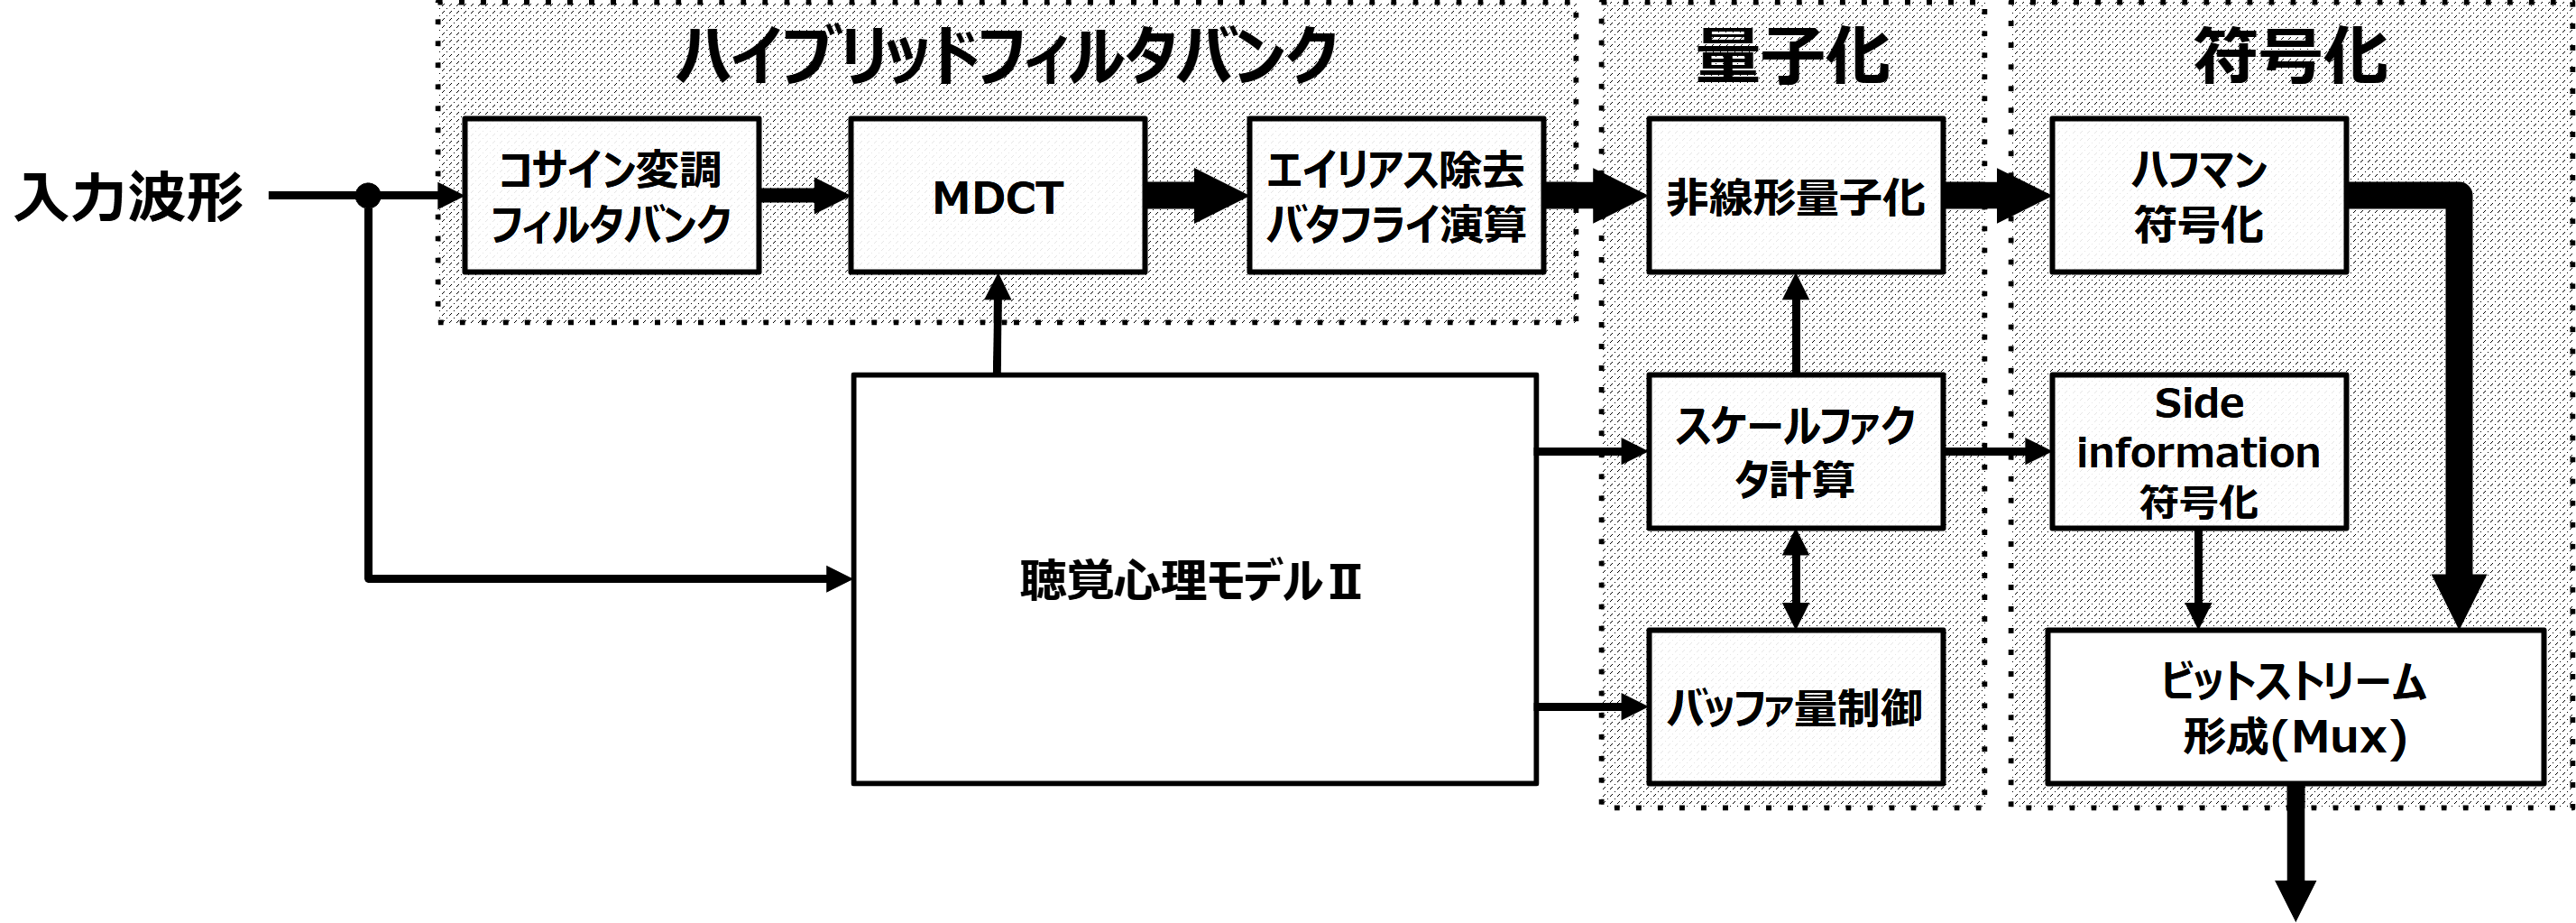
\includegraphics[width=115mm]{./figs/mp3_encoder_struct.png}
    \end{figure}
\end{frame}

\begin{frame}[c]
    \frametitle{MP3のデコーダ構造}
    \begin{figure}
        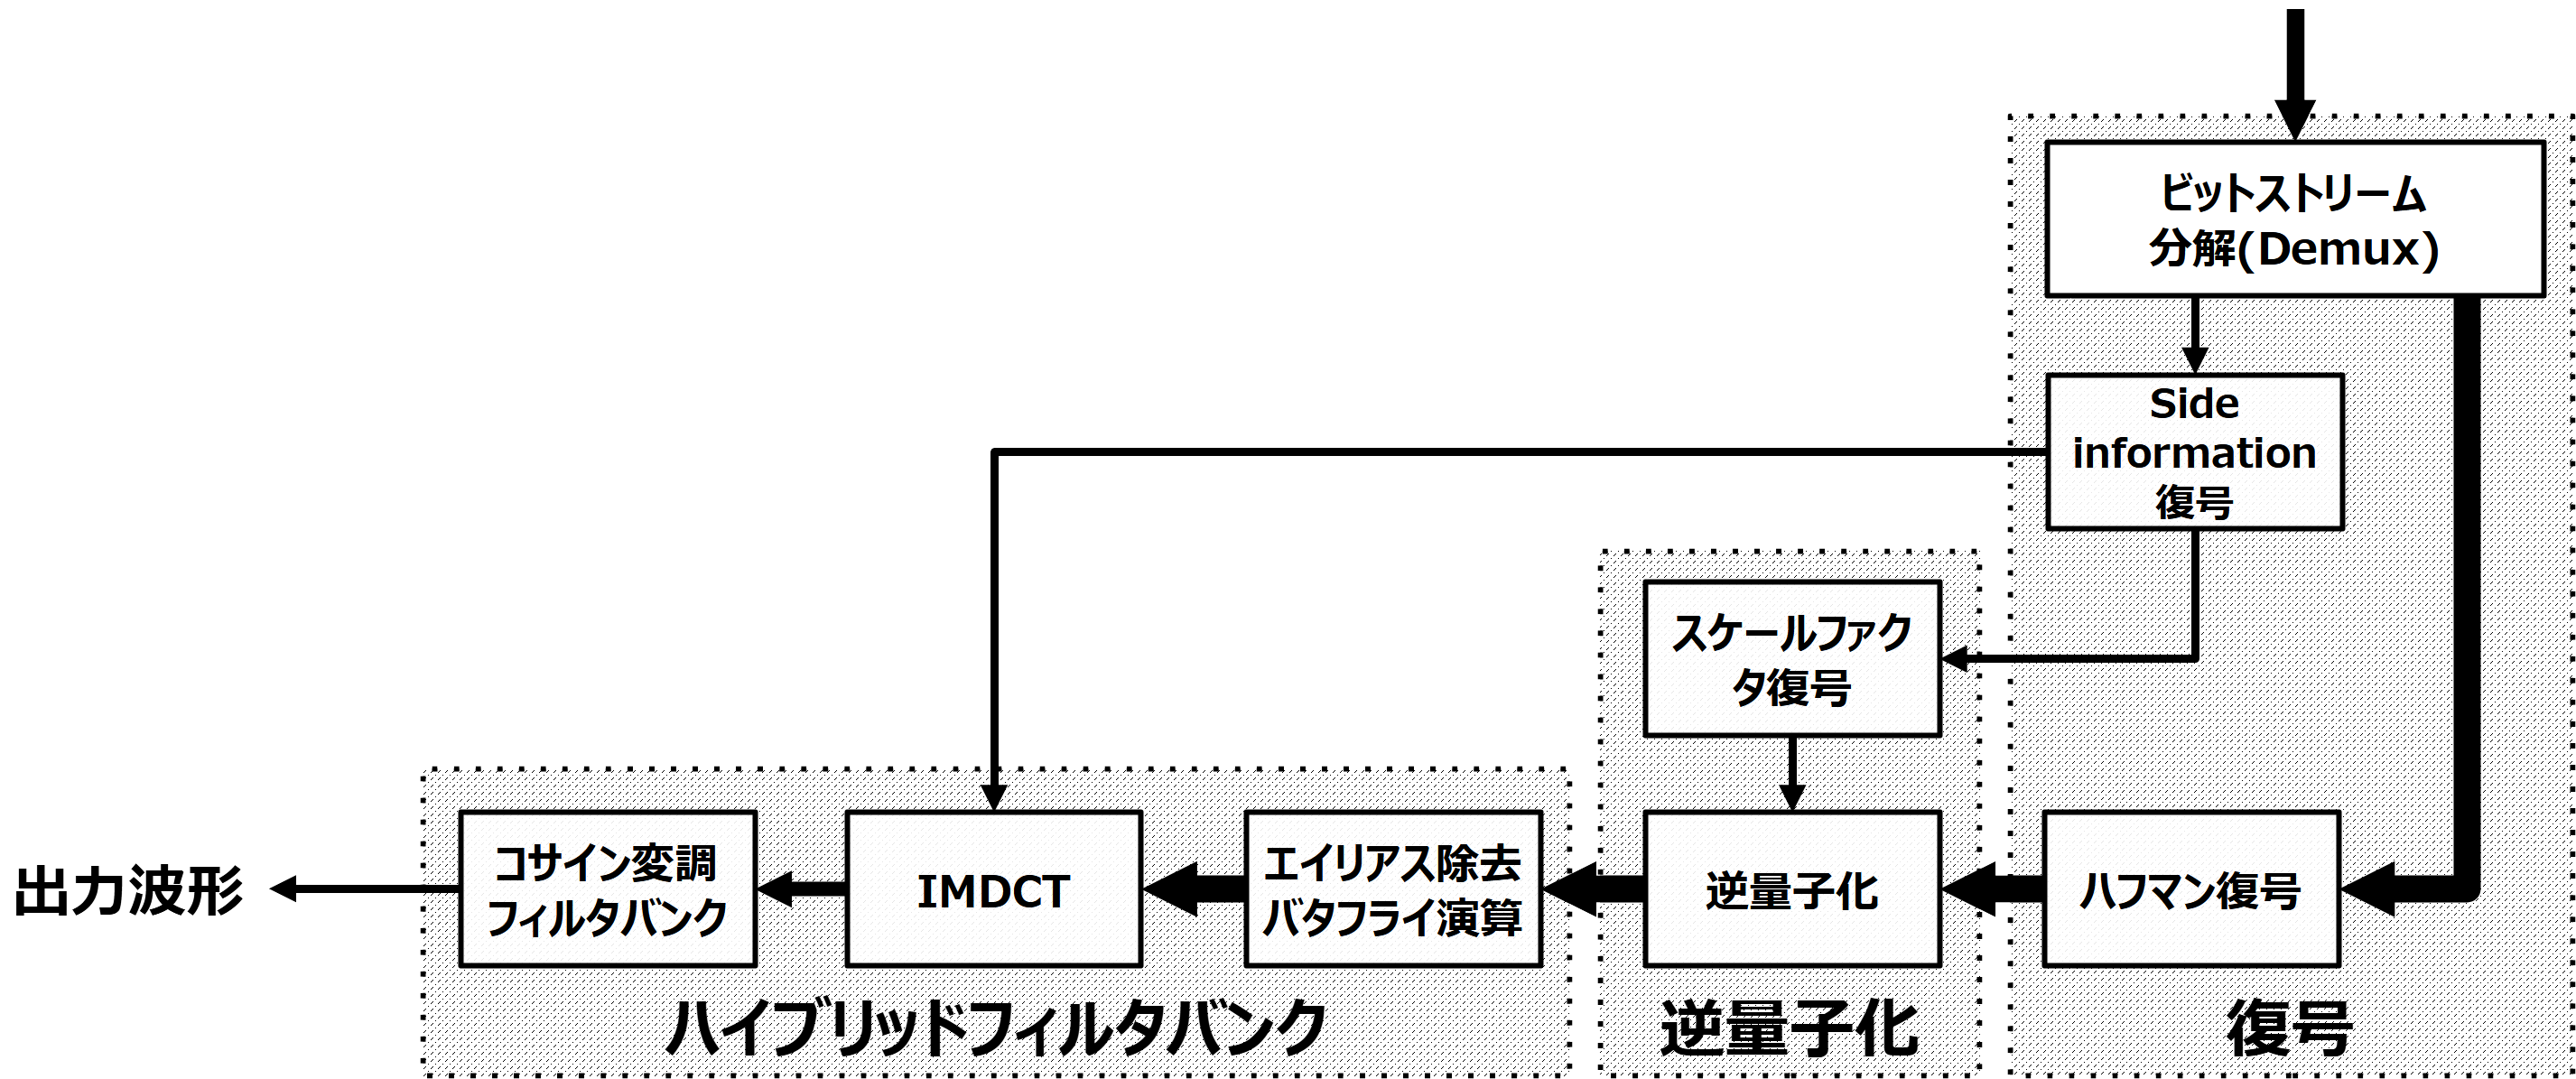
\includegraphics[width=115mm]{./figs/mp3_decoder_struct.png}
    \end{figure}
\end{frame}

\section{ハイブリッドフィルタバンク}

\subsection{コサイン変調フィルタバンク}

\begin{frame}[c]
    \frametitle{$M$分割フィルタバンク}
    \begin{figure}
        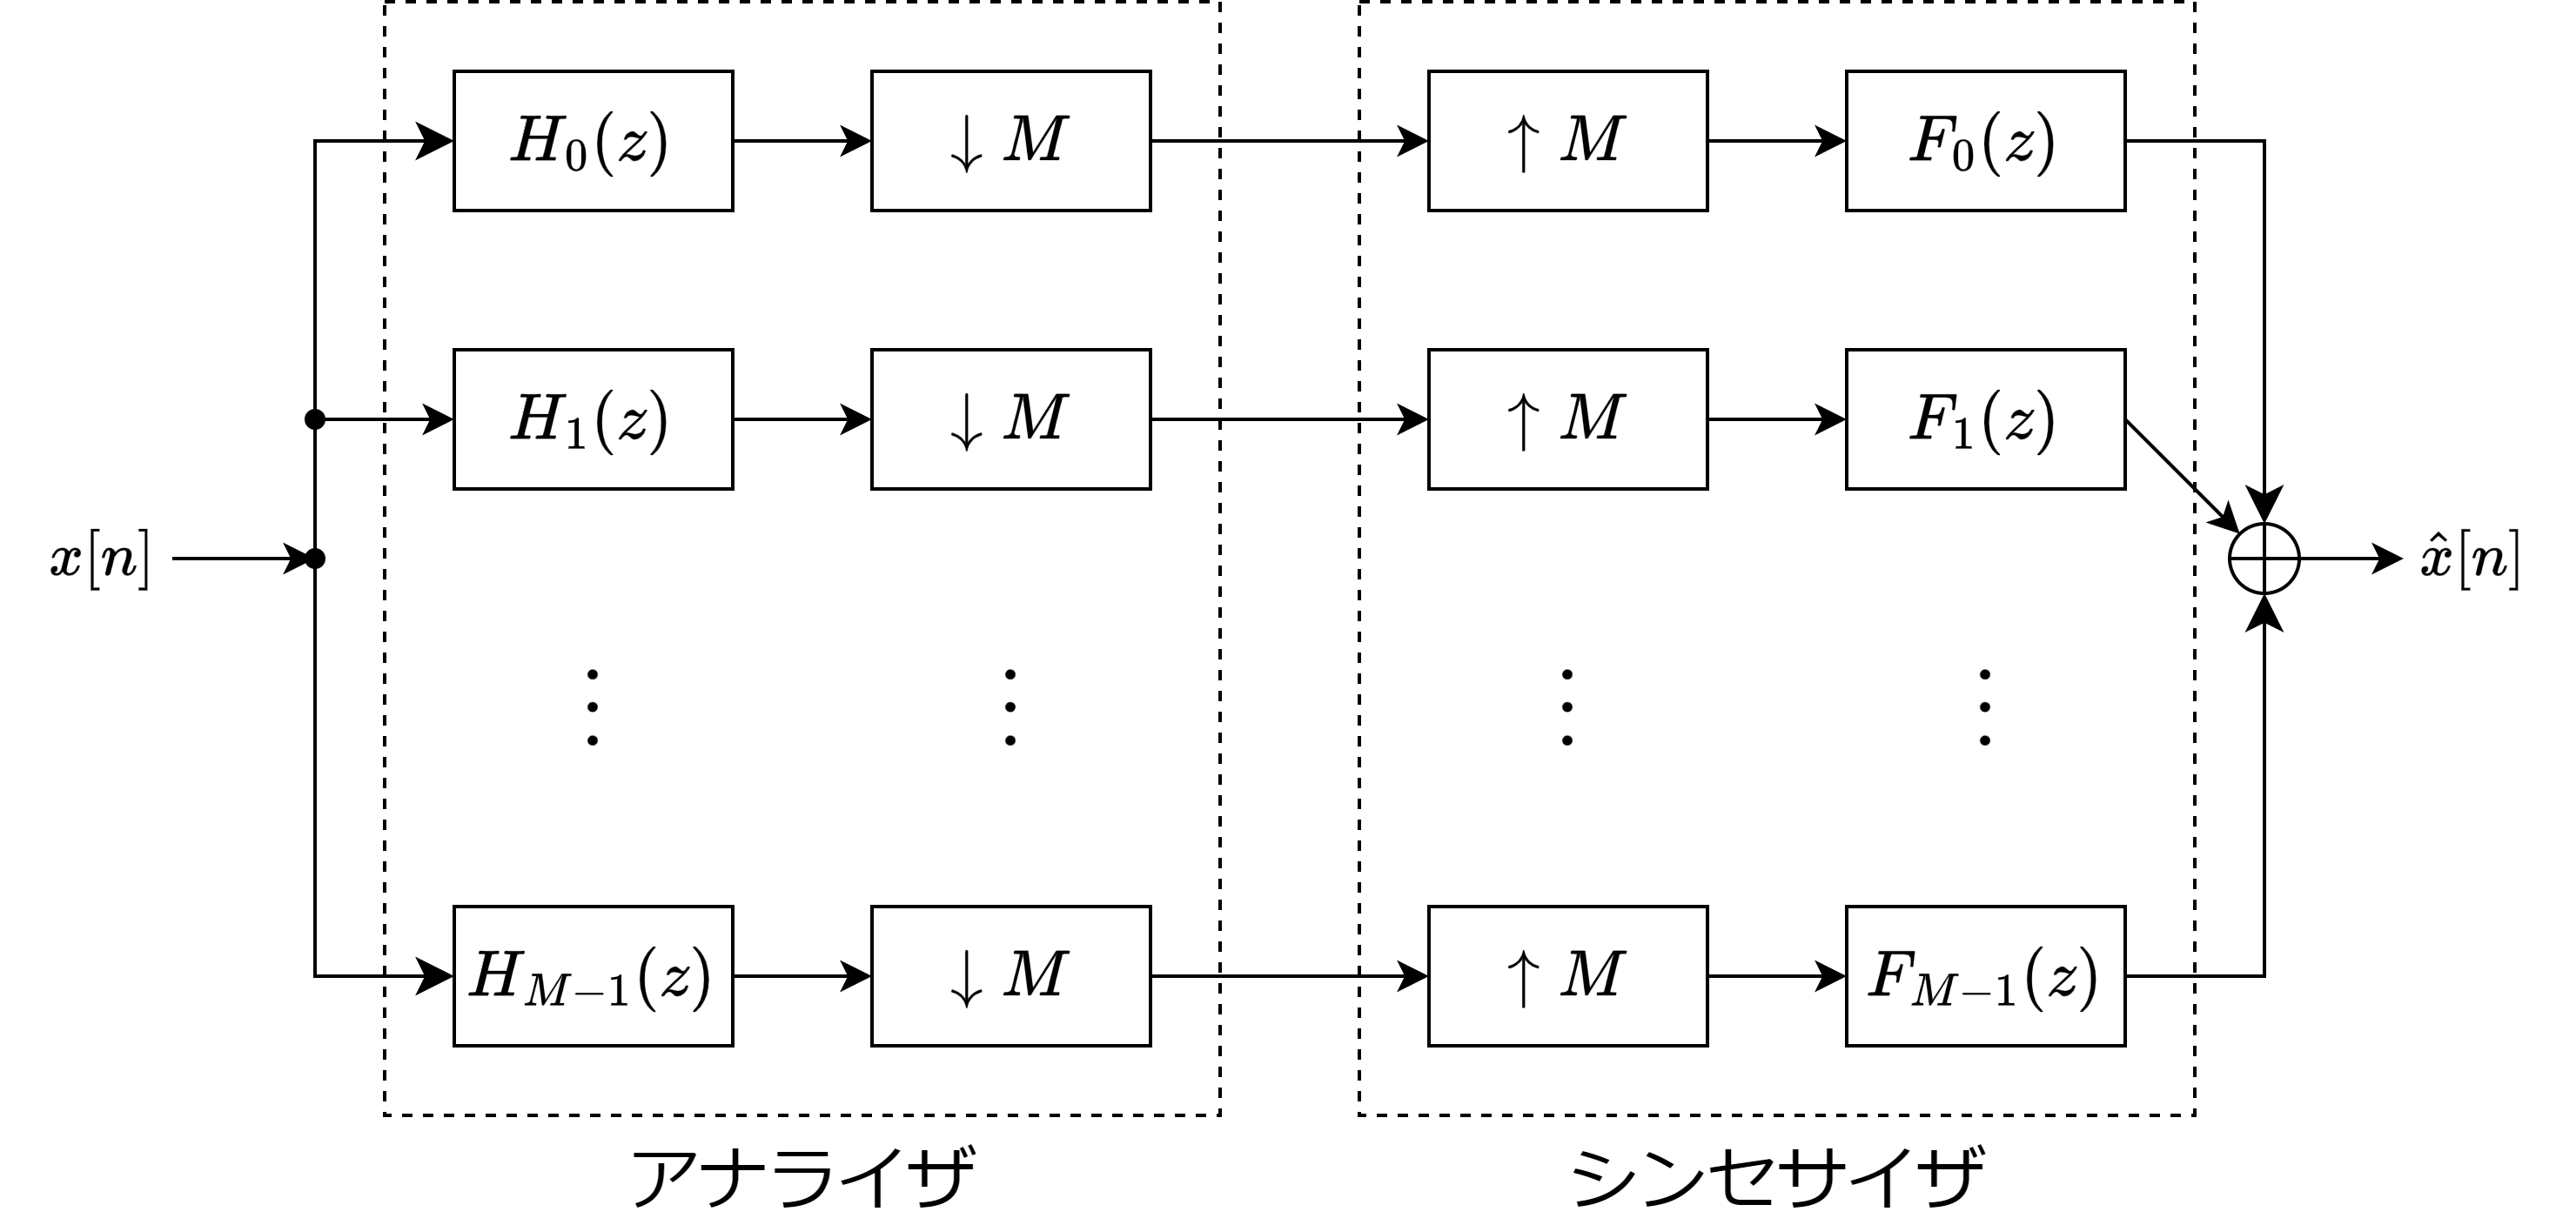
\includegraphics[width=120mm]{./figs/filter_bank.drawio.png}
    \end{figure}
\end{frame}

\begin{frame}[c]
    \frametitle{完全再構成}
    遅延・定数倍を除き入出力が一致すること:
    \begin{align}
        \hat{x}[n] = c x[n - n_{0}] \quad c \neq 0
    \end{align}
    $z$領域で,
    \begin{align}
        \hat{X}(z) = c z^{-n_{0}} X(z)
    \end{align}
    となること
    \begin{block}{}
        どんなどきに,$M$分割フィルタバンクが完全再構成になるか?(完全再構成条件→証明は補足(\ref{sec:proofs_filter_bank}節)
    \end{block}
\end{frame}

\begin{frame}[c]
    \frametitle{コサイン変調フィルタバンク}
    \begin{block}{コサイン変調フィルタバンク}
        \vspace{-10pt}
        \begin{align}
            h_{k}[n] &= 2 p_{0}[n] \cos \left[ \frac{\pi}{M} \left( k + \frac{1}{2} \right) \left( n - \frac{L - 1}{2} + \theta_{k} \right) \right] \label{eq:cos_modulated_analysis_filter} \\
            f_{k}[n] &= h_{k}[L - 1 - n] \label{eq:cos_modulated_synthesis_filter}
        \end{align}
        $M$:分割帯域数,$L$:タップ長,$\theta_{k} = (-1)^{k} \frac{\pi}{4}$
    \end{block}
    \begin{itemize}
        \item 1つの実係数・直線位相\structure{プロトタイプフィルタ}$p_{0}[n]$をコサインで変調して他のフィルタを設定
        % \item $p_{0}[n]$をうまく設計することで,アナライザ$H_{k}(z)$,シンセサイザ$F_{k}(z)$を実係数FIRフィルタとできる
    \end{itemize}
\end{frame}

\begin{frame}[c]
    \frametitle{コサイン変調フィルタバンク}
    \begin{block}{コサイン変調フィルタバンクの完全再構成条件}
        $k = 0, ..., M-1$に対し,定数$\alpha \in \mathbb{R}$があって
        \begin{align}
            G_{k}(z^{-1}) G_{k}(z) + G_{M + k}(z^{-1}) G_{M + k}(z) = \alpha \quad 
        \end{align}
        となること.ここで,
        \begin{align}
            G_{k}(z) = \sum_{n = -\infty}^{\infty} p_{0}[2Mn + k] z^{-n} \label{eq:polyphase_representation_of_prototype}
        \end{align}
        $G_{k}(z)$は$p_{0}[n]$のポリフェーズ表現という
    \end{block}
    本条件は\structure{電力相補条件}ともいう
\end{frame}

\begin{frame}[c]
    \frametitle{MP3のフィルタバンク}
    \begin{block}{MP3のフィルタバンク}
        \vspace{-10pt}
        \begin{align}
            y_{k}[t] &= \sum_{l = 0}^{511} x[t - l] h[l] \cos\left[ \frac{\pi}{32}\left( k + \frac{1}{2} \right) \left( l - 16 \right) \right] \\
            h[l] &= \left\{ \begin{array}{ll}
                -C_{l} & \lfloor l / 64 \rfloor \text{が偶数} \\
                 C_{l} & \lfloor l / 64 \rfloor \text{が奇数} \\
            \end{array} \right.
        \end{align}
        $C_{l}\ (l = 0,...,511)$は規格で設定
    \end{block}
    $M = 32, L = 33$としたコサイン変調フィルタバンク
\end{frame}

\begin{frame}[c]
    \frametitle{フィルタバンクの特性}
    \vspace{-5pt}
    \begin{figure}
        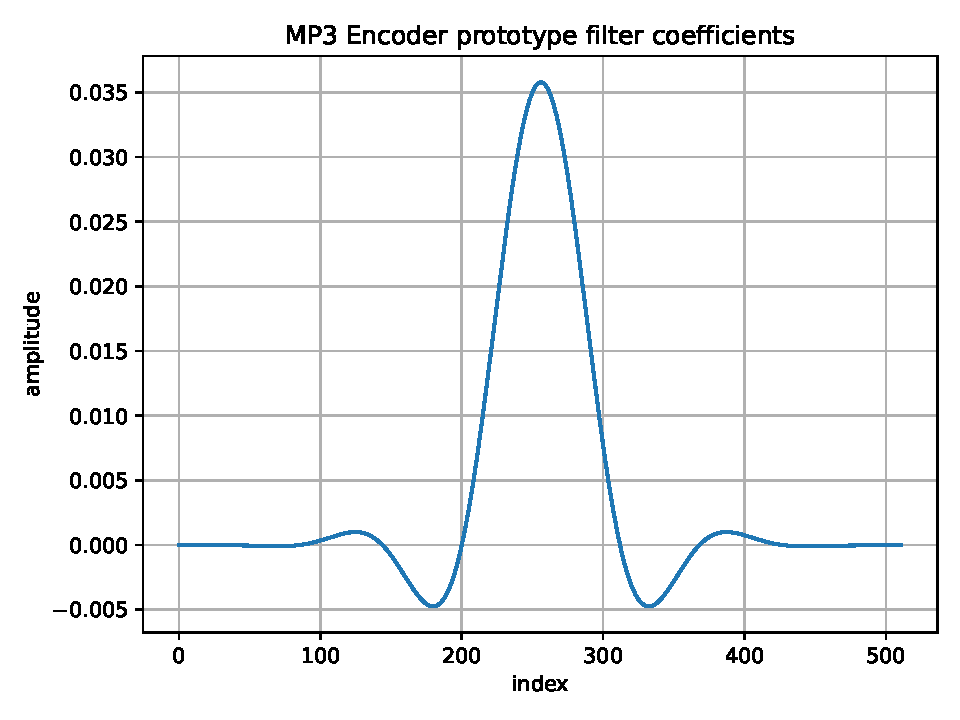
\includegraphics[width=100mm]{./figs/mp3_encoder_prototype_filter_coef.pdf}
    \end{figure}
    \vspace{-5pt}
    \begin{itemize}
        \item $h$の概形.対称で直線位相特性をもつ.
    \end{itemize}
\end{frame}

\begin{frame}[c]
    \frametitle{フィルタバンクの周波数特性}
    バンク$k = 0, ..., 15$の周波数特性
    \vspace{-5pt}
    \begin{figure}
        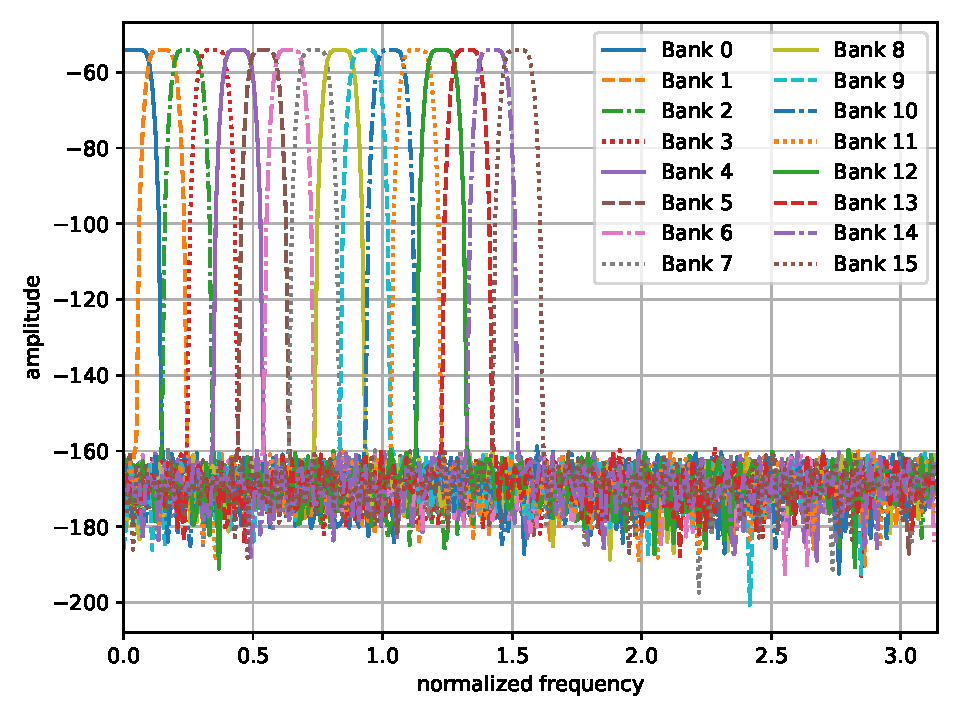
\includegraphics[width=105mm]{./figs/mp3_encoder_filter_bank_frequency_spec_0_15.pdf}
    \end{figure}
\end{frame}

\begin{frame}[c]
    \frametitle{フィルタバンクの周波数特性}
    バンク$k = 16, ..., 31$の周波数特性
    \vspace{-5pt}
    \begin{figure}
        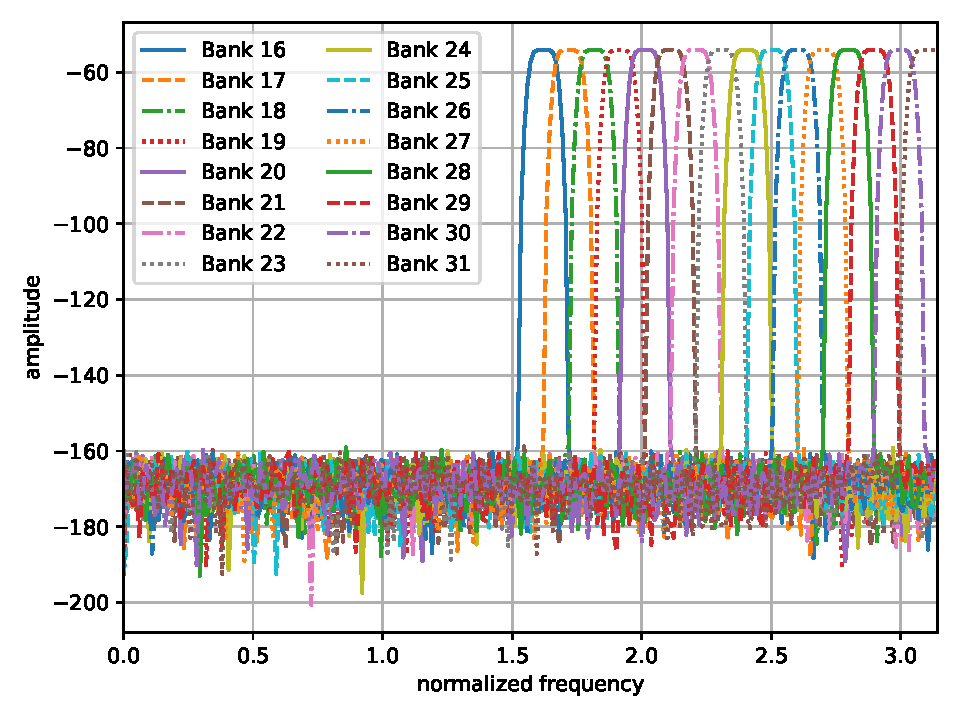
\includegraphics[width=105mm]{./figs/mp3_encoder_filter_bank_frequency_spec_16_31.pdf}
    \end{figure}
\end{frame}

\begin{frame}[c]
    \frametitle{フィルタバンクの実装}
    プログラムでは,
    \begin{align*}
        y_{k}[t] &= \sum_{s = 0}^{63} t_{k,s} \sum_{u = 0}^{7} x[t - s - 64u] C_{s + 64u} \\
        t_{k,s} &:= \cos\left[ \frac{\pi}{32}\left( k + \frac{1}{2} \right) \left( s - 16 \right) \right]
    \end{align*}
    で計算.この式が定義式通りであることを示す.
\end{frame}

\begin{frame}[c]
    \frametitle{フィルタバンクの実装}
    \scriptsize
    \begin{align}
        y_{k}[t] &= \sum_{l = 0}^{511} x[t - l] h[l] t_{k,l} = \sum_{u = 0}^{7} \sum_{s = 0}^{63} x[t - s - 64u] h[s + 64u] t_{k,s+64u} \nonumber \\
        &= \sum_{u = 0}^{7} \sum_{s = 0}^{63} x[t - s - 64u] (-1)^{u} C_{s + 64u} t_{k,s+64u} \label{eq:mp3_filterbank_progaram_deviation}
    \end{align}
    ここで,
    \begin{align*}
        t_{k,s+64u} &= \cos\left[ \frac{\pi}{32} \left( k + \frac{1}{2} \right) (s + 64u - 16) \right] = \cos\left[ \frac{\pi}{32} \left( k + \frac{1}{2} \right) (s - 16) + \pi \left( 2k + 1 \right) u \right] \\
        &= \cos\left[ \frac{\pi}{32} \left( k + \frac{1}{2} \right) (s - 16) \right]\cos\left[ \pi(2k + 1)u \right] \\
        &\quad - \sin\left[ \frac{\pi}{32} \left( k + \frac{1}{2} \right) (s - 16) \right]\sin\left[ \pi(2k + 1)u \right]
        % &= (-1)^{u} \cos\left[ \frac{\pi}{32} \left( k + \frac{1}{2} \right) (s - 16) \right] = (-1)^{u} 
        = (-1)^{u} t_{k,s}
    \end{align*}
    だから,これを式\eqref{eq:mp3_filterbank_progaram_deviation}に代入すれば,
    \begin{align*}
        y_{k}[t] = \sum_{u = 0}^{7} \sum_{s = 0}^{63} x[t - s - 64u] C_{s + 64u} t_{k,s} = \sum_{s = 0}^{63} t_{k,s} \sum_{u = 0}^{7} x[t - s - 64u] C_{s + 64u}
    \end{align*}
\end{frame}

\begin{frame}[c]
    \frametitle{電力相補条件の確認}
    MP3のフィルタバンクでは
    \scriptsize
    \begin{align*}
        G_{k}(z) &= \sum_{n = -\infty}^{\infty} h[2nM + k] z^{-n} = \sum_{n = 0}^{7} h[64n + k] z^{-n} = \sum_{n = 0}^{7} (-1)^{n} C_{64 + k} z^{-n} \\
        G_{M+k}(z) &= \sum_{n = 0}^{7} h[64n + 32 + k] z^{-n} = \sum_{n = 0}^{7} (-1)^{n} C_{64n + 32 + k} z^{-n} \\
        G_{k}(z^{-1}) &= \sum_{n = -\infty}^{\infty} h[64n + k] (z^{-1})^{-n} = \sum_{n = -\infty}^{\infty} h[-64n + k] z^{-n} = \sum_{n = -7}^{0} (-1)^{n} C_{-64n + k} z^{-n} \\
        G_{M+k}(z^{-1}) &= \sum_{n = 0}^{7} h[-64n + 32 + k] z^{-n} = \sum_{n = 0}^{7} (-1)^{n} C_{-64n + 32 + k} z^{-n}
    \end{align*}
    \normalsize
   $k = 0, ..., 31$で実際に計算すると,
    \begin{align*}
        G_{k}(z^{-1})G_{k}(z) + G_{M+k}(z^{-1})G_{M+k}(z) \approx \frac{1}{512}
    \end{align*}
\end{frame}

\begin{frame}[c]
    \frametitle{電力相補条件の確認(計算結果)}
    \begin{figure}
        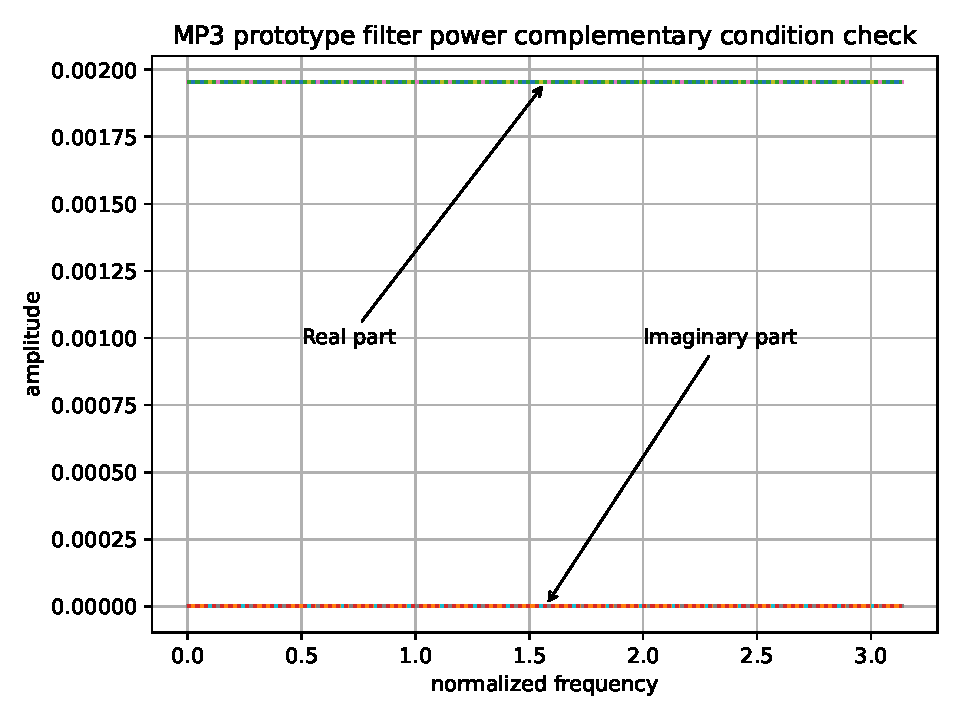
\includegraphics[width=115mm]{./figs/mp3_encoder_prototype_filter_power_complementary_condition.pdf}
    \end{figure}
\end{frame}

\subsection{MDCT}

\begin{frame}[c]
    \frametitle{MDCT}
    \begin{itemize}
        \item 変換式
        \item Princen-Bladrey条件
        \item MP3のブロックサイズ切り替え()
    \end{itemize}
\end{frame}

\begin{frame}[c]
    \frametitle{MDCT}
\end{frame}

\subsection{エイリアス削除バタフライ演算}

\begin{frame}[c]
    \frametitle{エイリアス削除バタフライ演算}
    処理と周波数特性の表示で十分(理論的なことはあまりないため)
\end{frame}

\section{量子化}

\begin{frame}[c]
    \frametitle{非線形量子化}
\end{frame}

\section{符号化}

\begin{frame}[c]
    \frametitle{ハフマン符号}
\end{frame}

\section{聴覚モデル}

\begin{frame}[c]
    \frametitle{聴覚モデル}
\end{frame}

\appendix

\section{証明}

\subsection{フィルタバンク} \label{sec:proofs_filter_bank}

\begin{frame}[c]
    \frametitle{ポリフェーズ表現}
    $H_{k}(z)$のインパルス応答を$h_{k}[n]$と書くとき,
    \small
    \begin{align*}
        H_{k}(z) &= \sum_{n = -\infty}^{\infty} h_{k}[n] z^{-n} = \sum_{n = -\infty}^{\infty} \sum_{l = 0}^{M - 1} h_{k}[nM + l] z^{-(nM+l)} \\
        &= \sum_{l = 0}^{M - 1} z^{-l} \sum_{n = -\infty}^{\infty}h_{k}[nM + l] z^{-nM} \\
        &= \sum_{l = 0}^{M - 1} E_{k,l}(z^{M}) z^{-l}
    \end{align*}
    \normalsize
    \begin{block}{$h_{k}$の(タイプI)ポリフェーズ表現}
        \vspace{-13pt}
        \begin{align}
            E_{k,l}(z) = \sum_{n = -\infty}^{\infty} h_{k}[nM + l] z^{-n} \label{eq:type1_polyphase_representation}
        \end{align}
    \end{block}
\end{frame}

\begin{frame}[c]
    \frametitle{ポリフェーズ表現}
    $F_{k}(z)$のインパルス応答を$f_{k}[n]$と書くとき,
    \scriptsize
    \begin{align*}
        F_{k}(z) &= \sum_{n = -\infty}^{\infty} f_{k}[n] z^{-n} = \sum_{n = -\infty}^{\infty} \sum_{l = 0}^{M - 1} f_{k}[nM + l] z^{-(nM+l)} \\
        &= \sum_{n = -\infty}^{\infty} \sum_{l^{\prime} = 0}^{M - 1} f_{k}[nM + M - 1 - l^{\prime}] z^{-(nM + M - 1 - l^{\prime})} \\
        &= \sum_{l^{\prime} = 0}^{M - 1} z^{-(M - 1 - l^{\prime})} \sum_{n = -\infty}^{\infty} f_{k}[nM + M - 1 - l^{\prime}] z^{-nM} = \sum_{l^{\prime} = 0}^{M - 1} z^{-(M - 1 - l^{\prime})} R_{k,l}(z^{M})
    \end{align*}
    \normalsize
    \begin{block}{$f_{k}$の(タイプII)ポリフェーズ表現}
        \vspace{-13pt}
        \begin{align}
            R_{k,l}(z) = \sum_{n = -\infty}^{\infty} f_{k}[nM + M - 1 - l] z^{-n} \label{eq:type2_polyphase_representation}
        \end{align}
    \end{block}
\end{frame}

\begin{frame}[c]
    \frametitle{ポリフェーズ行列表現}
    \eqref{eq:type1_polyphase_representation}式を$l$について並べ,行列表現すると
    \scriptsize
    \begin{align*}
        \underbrace{\begin{bNiceMatrix}[margin, nullify-dots, xdots/shorten=0.5em]
            H_{0}(z) \\
            H_{1}(z) \\
            \Vdots \\
            H_{M-1}(z)
        \end{bNiceMatrix}}_{\text{\normalsize $\ve{h}(z)$}}
        =
        \underbrace{\begin{bNiceMatrix}[margin, nullify-dots, xdots/shorten=0.5em]
              E_{0,0}(z^{M}) &   E_{0,1}(z^{M}) & \Cdots &   E_{0,M-1}(z^{M}) \\
              E_{1,0}(z^{M}) &   E_{1,1}(z^{M}) & \Cdots &   E_{1,M-1}(z^{M}) \\
                      \Vdots &           \Vdots & \Ddots &            \Vdots  \\
            E_{M-1,0}(z^{M}) & E_{M-1,1}(z^{M}) & \Cdots & E_{M-1,M-1}(z^{M}) \\
        \end{bNiceMatrix}}_{\text{\normalsize $\ve{E}(z)$}}
        \underbrace{\begin{bNiceMatrix}[margin, nullify-dots, xdots/shorten=0.5em]
                     1 \\
                z^{-1} \\
                \Vdots \\
            z^{-(M-1)}
        \end{bNiceMatrix}}_{\text{\normalsize $\ve{e}(z)$}}
    \end{align*}
    \normalsize
    \eqref{eq:type2_polyphase_representation}式も同様にして,以下のように書ける
    \scriptsize
    \begin{align*}
        \underbrace{\begin{bNiceMatrix}[margin, nullify-dots, xdots/shorten=0.5em]
            F_{0}(z) \\
            F_{1}(z) \\
            \Vdots \\
            F_{M-1}(z)
        \end{bNiceMatrix}}_{\text{\normalsize $\ve{f}(z)$}}
        =
        \underbrace{\begin{bNiceMatrix}[margin, nullify-dots, xdots/shorten=0.5em]
              R_{0,0}(z^{M}) &   R_{0,1}(z^{M}) & \Cdots &   R_{0,M-1}(z^{M}) \\
              R_{1,0}(z^{M}) &   R_{1,1}(z^{M}) & \Cdots &   R_{1,M-1}(z^{M}) \\
                      \Vdots &           \Vdots & \Ddots &            \Vdots  \\
            R_{M-1,0}(z^{M}) & R_{M-1,1}(z^{M}) & \Cdots & R_{M-1,M-1}(z^{M}) \\
        \end{bNiceMatrix}^{\mathsf{T}}}_{\text{\normalsize $\ve{R}(z)^{\mathsf{T}}$}}
        \underbrace{\begin{bNiceMatrix}[margin, nullify-dots, xdots/shorten=0.5em]
            z^{-(M-1)} \\
          z^{-(M-1)+1} \\
                \Vdots \\
                     1
        \end{bNiceMatrix}}_{z^{-(M-1)}\ve{e}(z^{-1})}
    \end{align*}
\end{frame}

\begin{frame}[c]
    \frametitle{ポリフェーズ行列表現}
    $\tilde{\ve{e}}(z) = \ve{e}(z^{-1})^{\mathsf{T}}$とすると行列表現は
    \begin{align}
        \ve{h}(z) &= \ve{E}(z) \ve{e}(z) \\
        \ve{f}(z)^{\mathsf{T}} &= z^{-(M-1)} \tilde{\ve{e}}(z) \ve{R}(z)
    \end{align}
    とまとめられる.$\ve{E}(z), \ve{R}(z)$を\structure{ポリフェーズ行列}という
\end{frame}

\begin{frame}[c]
    \frametitle{ポリフェーズ行列表現}
    $\ve{E}(z), \ve{R}(z)$により,アナライザ・シンセサイザは以下のように変形できる
    \begin{figure}
        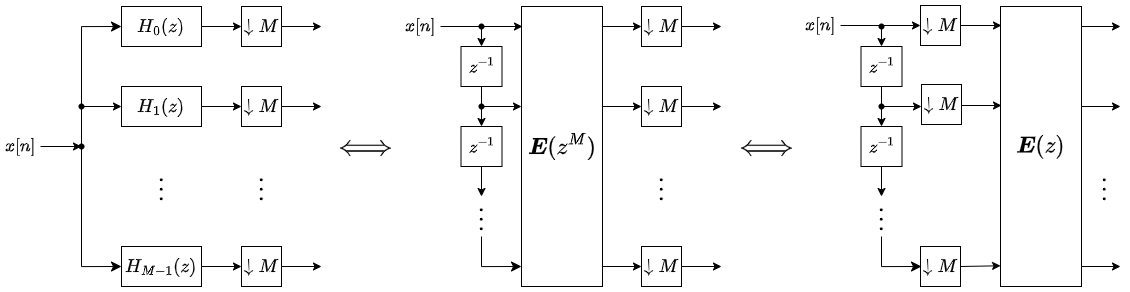
\includegraphics[width=118mm]{./figs/polyphase_representation_analyzer.drawio.png}
    \end{figure}
    \hrule
    \begin{figure}
        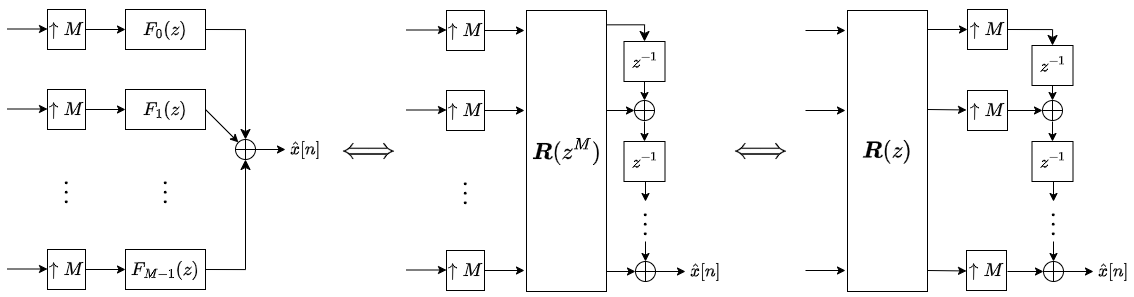
\includegraphics[width=118mm]{./figs/polyphase_representation_synthesizer.drawio.png}
    \end{figure}
\end{frame}

\begin{frame}[c]
    \frametitle{ポリフェーズ行列表現}
    $\ve{E}(z), \ve{R}(z)$により,$M$分割フィルタバンクは以下のように表せる
    \vspace{-13pt}
    \begin{figure}
        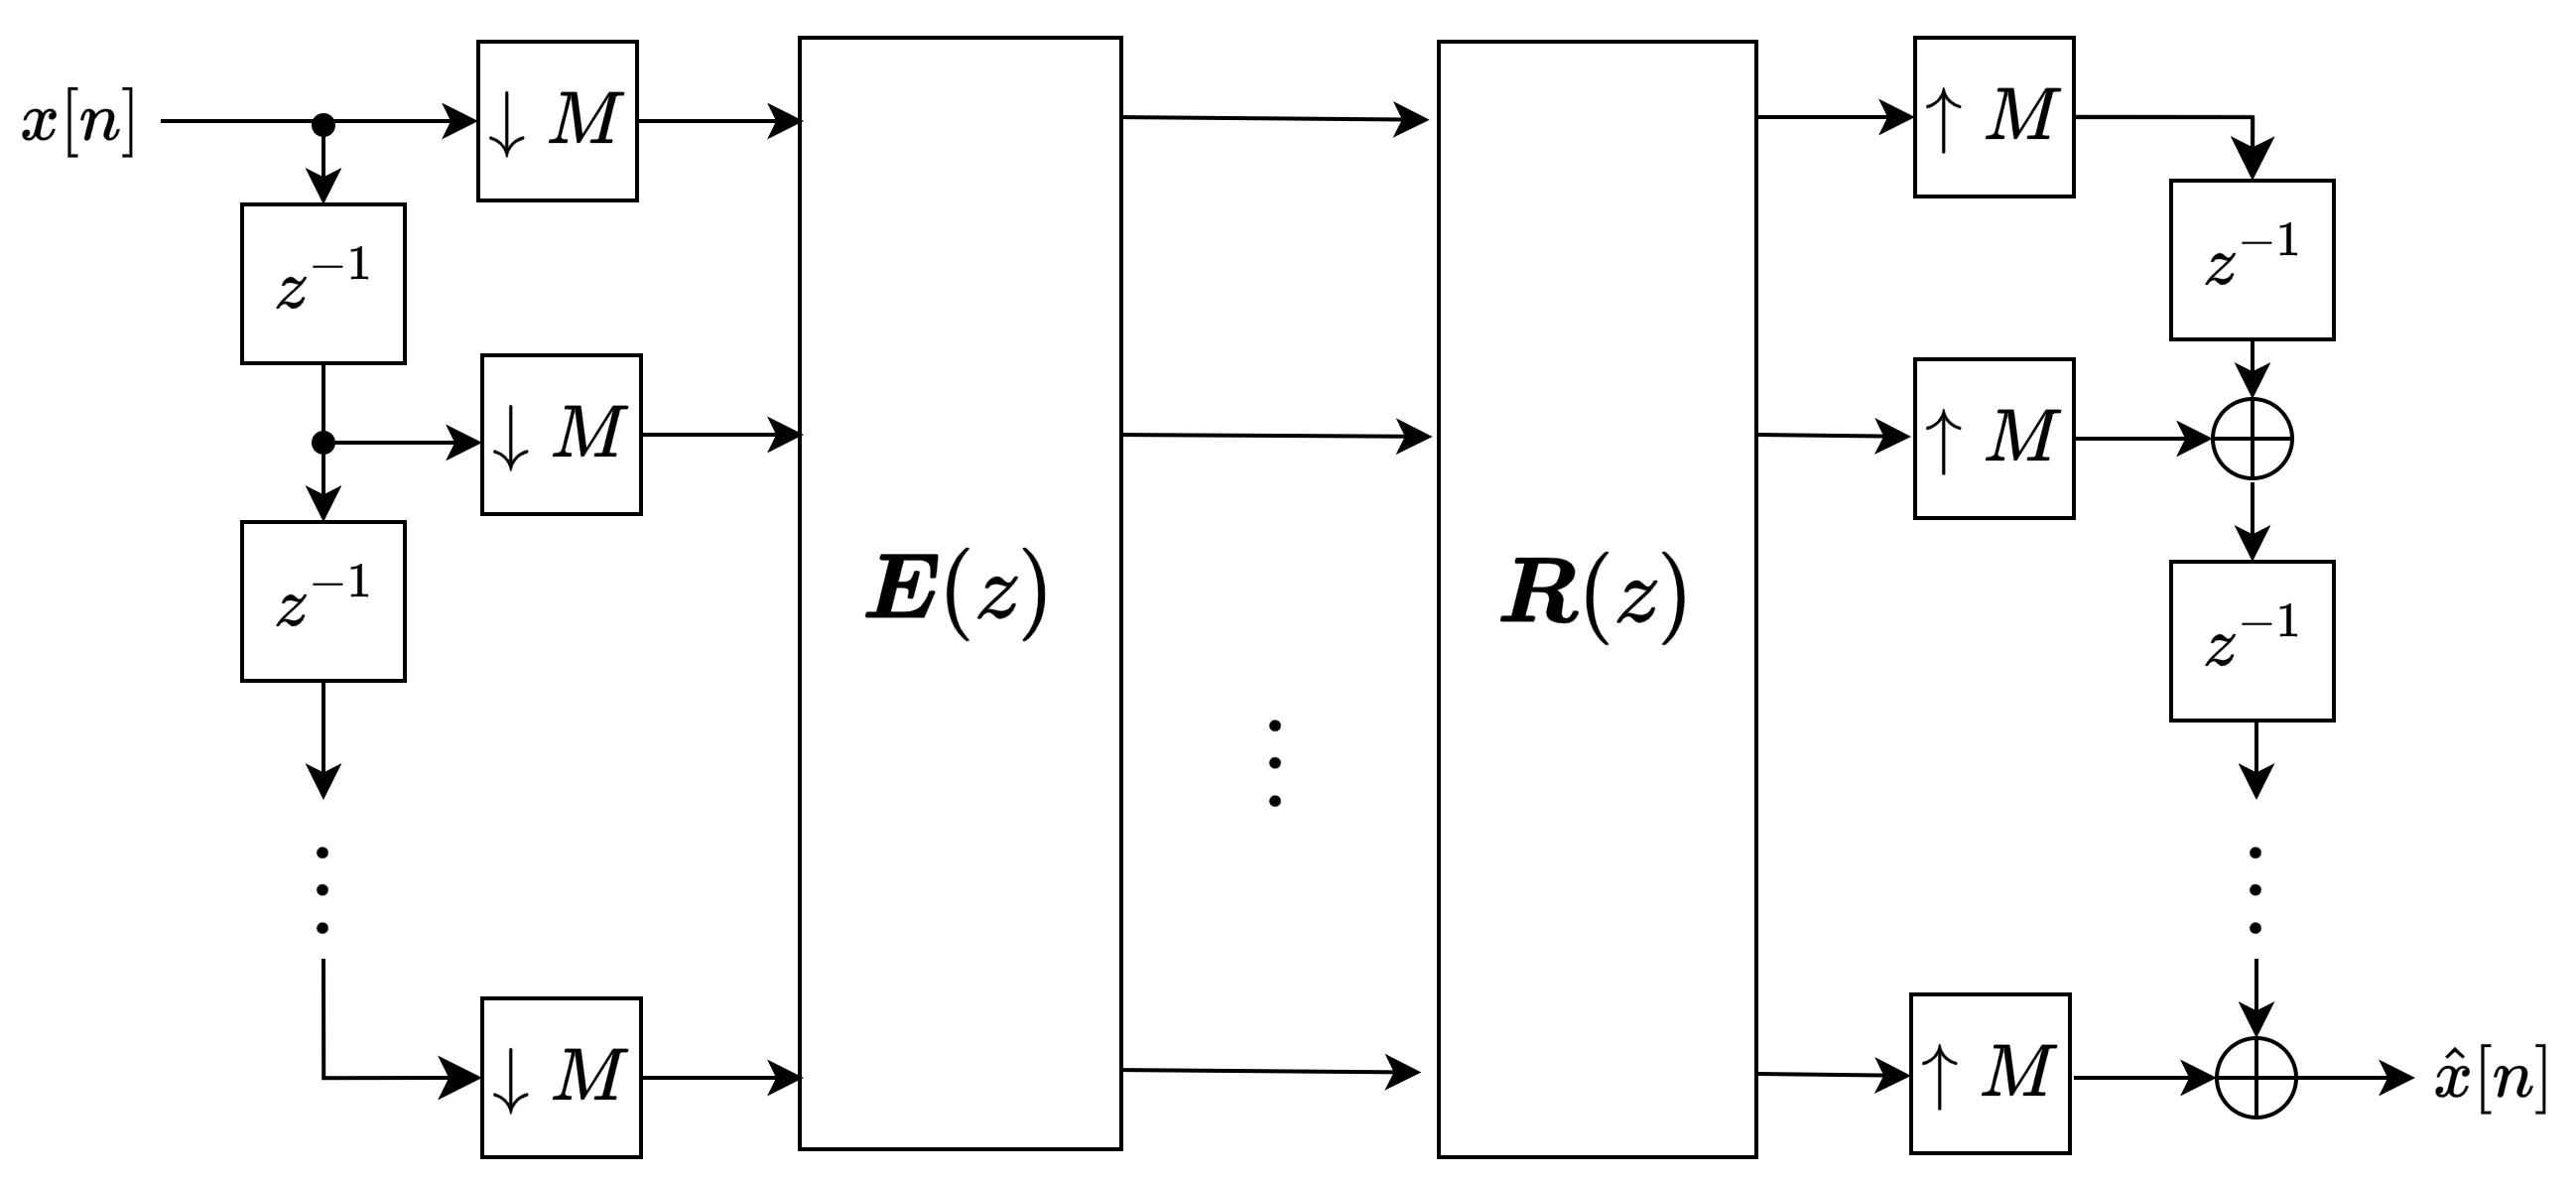
\includegraphics[width=120mm]{./figs/polyphase_representation_filter_bank.drawio.png}
    \end{figure}
\end{frame}

\begin{frame}[c]
    \frametitle{\scalebox{0.95}{完全再構成$M$分割フィルタバンク}}
    \begin{block}{}
        \vspace{-14pt}
        \begin{align}
            \ve{R}(z) \ve{E}(z) = a z^{-m_{0}} \ve{I} \quad (a \neq 0,\ m_{0} \in \mathbb{N}) \label{eq:filter_bank_PR_condition}
        \end{align}
        ならば,$M$分割フィルタバンクは完全再構成\footnote{$\because$各バンドの遅延が$K$ならば,$\hat{X}(z) = aM z^{-(M - 1 - K)}X(z)$}
    \end{block}
    \begin{figure}
        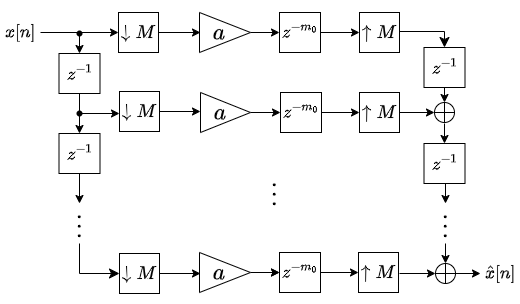
\includegraphics[width=70mm]{./figs/perfect_reconstraction_filter_bank.drawio.png}
        \caption*{$\ve{R}(z) \ve{E}(z) = a z^{-m_{0}} \ve{I}$を満たす$M$分割フィルタバンク}
    \end{figure}
\end{frame}

\begin{frame}[c]
    \frametitle{\scalebox{0.95}{完全再構成$M$分割フィルタバンク}}
    \eqref{eq:filter_bank_PR_condition}式より,$\ve{R}(z)$を
    \begin{align*}
        \ve{R}(z) = a z^{-m_{0}} \ve{E}(z)^{-1}
    \end{align*}
    とすれば完全再構成.しかし$\ve{E}(z)^{-1}$の計算が数値計算の安定性などの問題を孕む.
\end{frame}

\begin{frame}[c]
    \frametitle{\scalebox{0.95}{完全再構成$M$分割フィルタバンク}}
    $\ve{E}(z)^{-1}$の代わりに,$\ve{E}(z)$に\structure{パラユニタリ性}
    \begin{align}
        \widetilde{\ve{E}}(z) \ve{E}(z) = d \ve{I} \quad d \neq 0
    \end{align}
    を求める方法がある\footnote{$\widetilde{\ve{E}}(z) = \ve{E}_{\ast}(z^{-1})$で,下付きの$\ast$は係数の複素共役}.$\ve{E}(z)$がパラユニタリであれば,
    \begin{align*}
        \ve{R}(z) = a z^{-m_{0}} \widetilde{\ve{E}}(z)
    \end{align*}
    とすると完全再構成になる.
\end{frame}

\begin{frame}[c]
    \frametitle{コサイン変調フィルタバンク}
    \begin{block}{}
    式\eqref{eq:cos_modulated_synthesis_filter}より,分析合成フィルタ$F_{k}(z)H_{k}(z)$は直線位相特性をもつ
    \end{block}
    \scriptsize
    (証明)
    \begin{align*}
        F_{k}(z) &= \sum_{n = -\infty}^{\infty} f_{k}[n] z^{-n} = \sum_{n = -\infty}^{\infty} h_{k}[L - 1 - n] z^{-n} \\
        &= \sum_{n^{\prime} = -\infty}^{\infty} h_{k}[n^{\prime}] z^{-(L - 1 - n^{\prime})} = z^{-(L-1)} \sum_{n^{\prime} = -\infty}^{\infty} h_{k}[n^{\prime}] z^{n^{\prime}} \\
        &= z^{-(L-1)} H_{k}(z^{-1})
    \end{align*}
    $H_{k}(z)$の周波数特性を(極座標で)$H_{k}(\omega) = |H_{k}(\omega)| \exp[j \psi(\omega)]$と書くと,
    \begin{align*}
        F_{k}(\omega) &= \exp[-j(L - 1)\omega] H_{k}(-\omega) = \exp[-j(L - 1)\omega] |H_{k}(-\omega)| \exp[-j \psi(\omega)] \\
        &= \exp[-j(L - 1)\omega] |H_{k}(\omega)| \exp[-j \psi(\omega)] \quad \text{($\because$ 実係数FIRの振幅特性は偶)}
    \end{align*}
    だから,$F_{k}(\omega) H_{k}(\omega) = \exp[-j(L - 1)\omega] |H_{k}(\omega)|^{2}$となって直線位相特性をもつ.
\end{frame}

\begin{frame}[c]
    \frametitle{コサイン変調フィルタバンク}
    $h_{k}[n]$の伝達関数を変形する.回転因子$W_{2M}$\footnote{$W_{2M} = \exp\left(-j\frac{\pi}{M}\right)$}より
    \scriptsize
    \begin{align*}
        &\cos\left[ \frac{\pi}{M} \left( k + \frac{1}{2} \right) \left( n - \frac{L - 1}{2} + \theta_{k} \right) \right] \\
        &= \frac{1}{2} \left\{ \exp\left[ j \frac{\pi}{M} \left( k + \frac{1}{2} \right) \left( n - \frac{L - 1}{2} + \theta_{k} \right) \right] + \exp\left[-j \frac{\pi}{M} \left( k + \frac{1}{2} \right) \left( n - \frac{L - 1}{2} + \theta_{k} \right) \right] \right\} \\
        &= \frac{1}{2} \left\{ \exp(j\theta_{k}) W_{2M}^{\left( k + \frac{1}{2} \right)\frac{L-1}{2}}W_{2M}^{-\left( k + \frac{1}{2} \right)n} + \exp(-j\theta_{k}) W_{2M}^{-\left( k + \frac{1}{2} \right)\frac{L-1}{2}} W_{2M}^{\left( k + \frac{1}{2} \right)n} \right\}
    \end{align*}
    \normalsize
    これを\eqref{eq:cos_modulated_analysis_filter}式に代入すると,
    \scriptsize
    \begin{align*}
        H_{k}(z) &= \exp(j\theta_{k}) W_{2M}^{\left( k + \frac{1}{2} \right)\frac{L-1}{2}} \sum_{n = -\infty}^{\infty} p_{0}[n] W_{2M}^{-\left(k + \frac{1}{2} \right)n} z^{-n} \\
        &\quad + \exp(-j\theta_{k}) W_{2M}^{-\left( k + \frac{1}{2} \right)\frac{L-1}{2}} \sum_{n = -\infty}^{\infty} p_{0}[n] W_{2M}^{\left(k + \frac{1}{2} \right)n} z^{-n} \\
        &= \exp(j\theta_{k}) W_{2M}^{\left( k + \frac{1}{2} \right)\frac{L-1}{2}} P_{0}\left(W_{2M}^{k + \frac{1}{2}} z \right) + \exp(-j\theta_{k}) W_{2M}^{-\left( k + \frac{1}{2} \right)\frac{L-1}{2}} P_{0}\left(W_{2M}^{-\left(k + \frac{1}{2}\right)} z \right)
    \end{align*}
\end{frame}

\begin{frame}[c]
    \frametitle{コサイン変調フィルタバンク}
    さらに\eqref{eq:polyphase_representation_of_prototype}式を代入すると\footnote{$\left( W_{2M}^{\pm \left( k + \frac{1}{2} \right) }\right)^{2M} = \exp\left[ \mp j \frac{\pi}{M} \left( k + \frac{1}{2} \right) 2M \right] = \exp[\mp j \pi(2k + 1)] = -1$ を使用}
    \scriptsize
    \begin{align*}
        &H_{k}(z) = \exp(j\theta_{k}) W_{2M}^{\left( k + \frac{1}{2} \right)\frac{L-1}{2}} \sum_{l = 0}^{2M - 1} \left( W_{2M}^{k + \frac{1}{2}} z \right)^{-l} G_{l}\left( \left( W_{2M}^{k + \frac{1}{2}} z \right)^{2M} \right) \\
        &\quad\quad\quad + \exp(-j\theta_{k}) W_{2M}^{-\left( k + \frac{1}{2} \right)\frac{L-1}{2}} \sum_{l = 0}^{2M - 1} \left( W_{2M}^{-\left( k + \frac{1}{2} \right)} z \right)^{-l} G_{l}\left( \left( W_{2M}^{-\left( k + \frac{1}{2} \right)} z \right)^{2M} \right) \\
        &= \exp(j\theta_{k}) W_{2M}^{\left( k + \frac{1}{2} \right)\frac{L-1}{2}} \sum_{l = 0}^{2M - 1} W_{2M}^{-l\left( k + \frac{1}{2} \right)} z^{-l} G_{l}(-z^{2M}) \\
        &\quad\quad\quad + \exp(-j\theta_{k}) W_{2M}^{-\left( k + \frac{1}{2} \right)\frac{L-1}{2}} \sum_{l = 0}^{2M - 1} W_{2M}^{l\left( k + \frac{1}{2} \right)} z^{-l} G_{l}(-z^{2M}) \\
        &= 
        \scalebox{0.97}{$\displaystyle\sum_{l = 0}^{2M - 1} \left\{ \exp(j\theta_{k}) W_{2M}^{\left( k + \frac{1}{2} \right)\frac{L-1}{2}} W_{2M}^{-l\left( k + \frac{1}{2} \right)} + \exp(-j\theta_{k}) W_{2M}^{-\left( k + \frac{1}{2} \right)\frac{L-1}{2}}W_{2M}^{l\left( k + \frac{1}{2} \right)} \right\} z^{-l} G_{l}(-z^{2M})$}
        \\
        &= \sum_{l = 0}^{2M - 1} 2 \cos\left[ \frac{\pi}{M} \left( k + \frac{1}{2} \right) \left( l - \frac{L - 1}{2} \right) + \theta_{k} \right] z^{-l} G_{l}(-z^{2M})
    \end{align*}
\end{frame}

\begin{frame}[c]
    \frametitle{コサイン変調フィルタバンク}
    さらに変形すると
    \small
    \begin{align}
        H_{k}(z) &= \sum_{l = 0}^{M - 1} z^{-l} \left\{ t_{k,l} G_{l}(-z^{2M}) + z^{-M} t_{k,M + l} G_{M + l}(-z^{2M}) \right\} \label{eq:another_polyphase_representation} \\
        t_{k,l} &:= 2\cos\left[ \frac{\pi}{M} \left( k + \frac{1}{2} \right) \left( l - \frac{L - 1}{2} \right) + \theta_{k} \right] \nonumber
    \end{align}
    \normalsize
    \eqref{eq:type1_polyphase_representation}式と\eqref{eq:another_polyphase_representation}式を見比べると,
    \begin{align}
        E_{k, l}(z) = t_{k,l} G_{l}(-z^{2}) + z^{-1} t_{k,M + l} G_{M + l}(-z^{2}) \label{eq:polyphase_representation_of_cos_modulated_filter_bank}
    \end{align}
\end{frame}

\begin{frame}[c]
    \frametitle{コサイン変調フィルタバンク}
    \eqref{eq:polyphase_representation_of_cos_modulated_filter_bank}式より,アナライザのポリフェーズ行列は,
    \footnotesize
    \begin{align}
        \ve{E}(z) &= 
        \underbrace{\begin{bNiceMatrix}[margin, nullify-dots, xdots/shorten=0.5em]
              t_{0,0} & \Cdots &   t_{0,2M-1} \\
              t_{1,0} & \Cdots &   t_{1,2M-1} \\
               \Vdots & \Cdots &      \Vdots  \\
            t_{M-1,0} & \Cdots & t_{M-1,2M-1} \\
        \end{bNiceMatrix}}_{\ve{T}}
        \begin{bNiceMatrix}[margin, nullify-dots, xdots/shorten=0.5em]
                  G_{0}(-z^{2}) &        &                         \\
                                & \Ddots &                         \\
                                &        &         G_{M-1}(-z^{2}) \\
            z^{-1}G_{M}(-z^{2}) &        &                         \\
                                & \Ddots &                         \\
                                &        & z^{-1} G_{2M-1}(-z^{2}) \\
        \end{bNiceMatrix}
        \nonumber \\
        &= \ve{T}
        \begin{bNiceMatrix}[margin, nullify-dots, xdots/shorten=0.5em]
            \ve{G}_{0}(z^{2}) \\
            z^{-1} \ve{G}_{1}(z^{2}) \\
        \end{bNiceMatrix} \label{eq:analyzer_matrix_of_cos_modulated_filter_bank} \\
        \ve{G}_{i}(z) &:=
        \diag \begin{bNiceMatrix}[margin, nullify-dots, xdots/shorten=0.5em]
            G_{Mi}(-z) & G_{Mi + 1}(-z) & \Cdots & G_{Mi + M - 1}(-z)
        \end{bNiceMatrix}
    \end{align}
    \normalsize
    と書ける
\end{frame}

\begin{frame}[c]
    \frametitle{コサイン変調フィルタバンク}
    シンセサイザを構成する.フィルタ係数は実だから,
    \begin{align}
        \widetilde{\ve{E}}(z) = \ve{E}_{\ast}(z^{-1})^{\mathsf{T}} = 
        \begin{bNiceMatrix}[margin, nullify-dots, xdots/shorten=0.5em]
            \ve{G}_{0}(z^{-1}) & z \ve{G}_{1}(z^{-1})
        \end{bNiceMatrix}
        \ve{T}^{\mathsf{T}}
    \end{align}
    $G_{l}(z)$の次数は$2K - 1$で,因果性のためには$2K - 1$の遅延がいるため
    \begin{align}
        \ve{R}(z) &= z^{-(2K-1)} \widetilde{\ve{E}}(z) \nonumber \\
        &=
        z^{-(2K-1)} 
        \begin{bNiceMatrix}[margin, nullify-dots, xdots/shorten=0.5em]
            \ve{G}_{0}(z^{-1}) & z \ve{G}_{1}(z^{-1})
        \end{bNiceMatrix}
        \ve{T}^{\mathsf{T}} \label{eq:synthesizer_matrix_of_cos_modulated_filter_bank}
    \end{align}
\end{frame}

\begin{frame}[c]
    \frametitle{コサイン変調フィルタバンク}
    \begin{figure}
        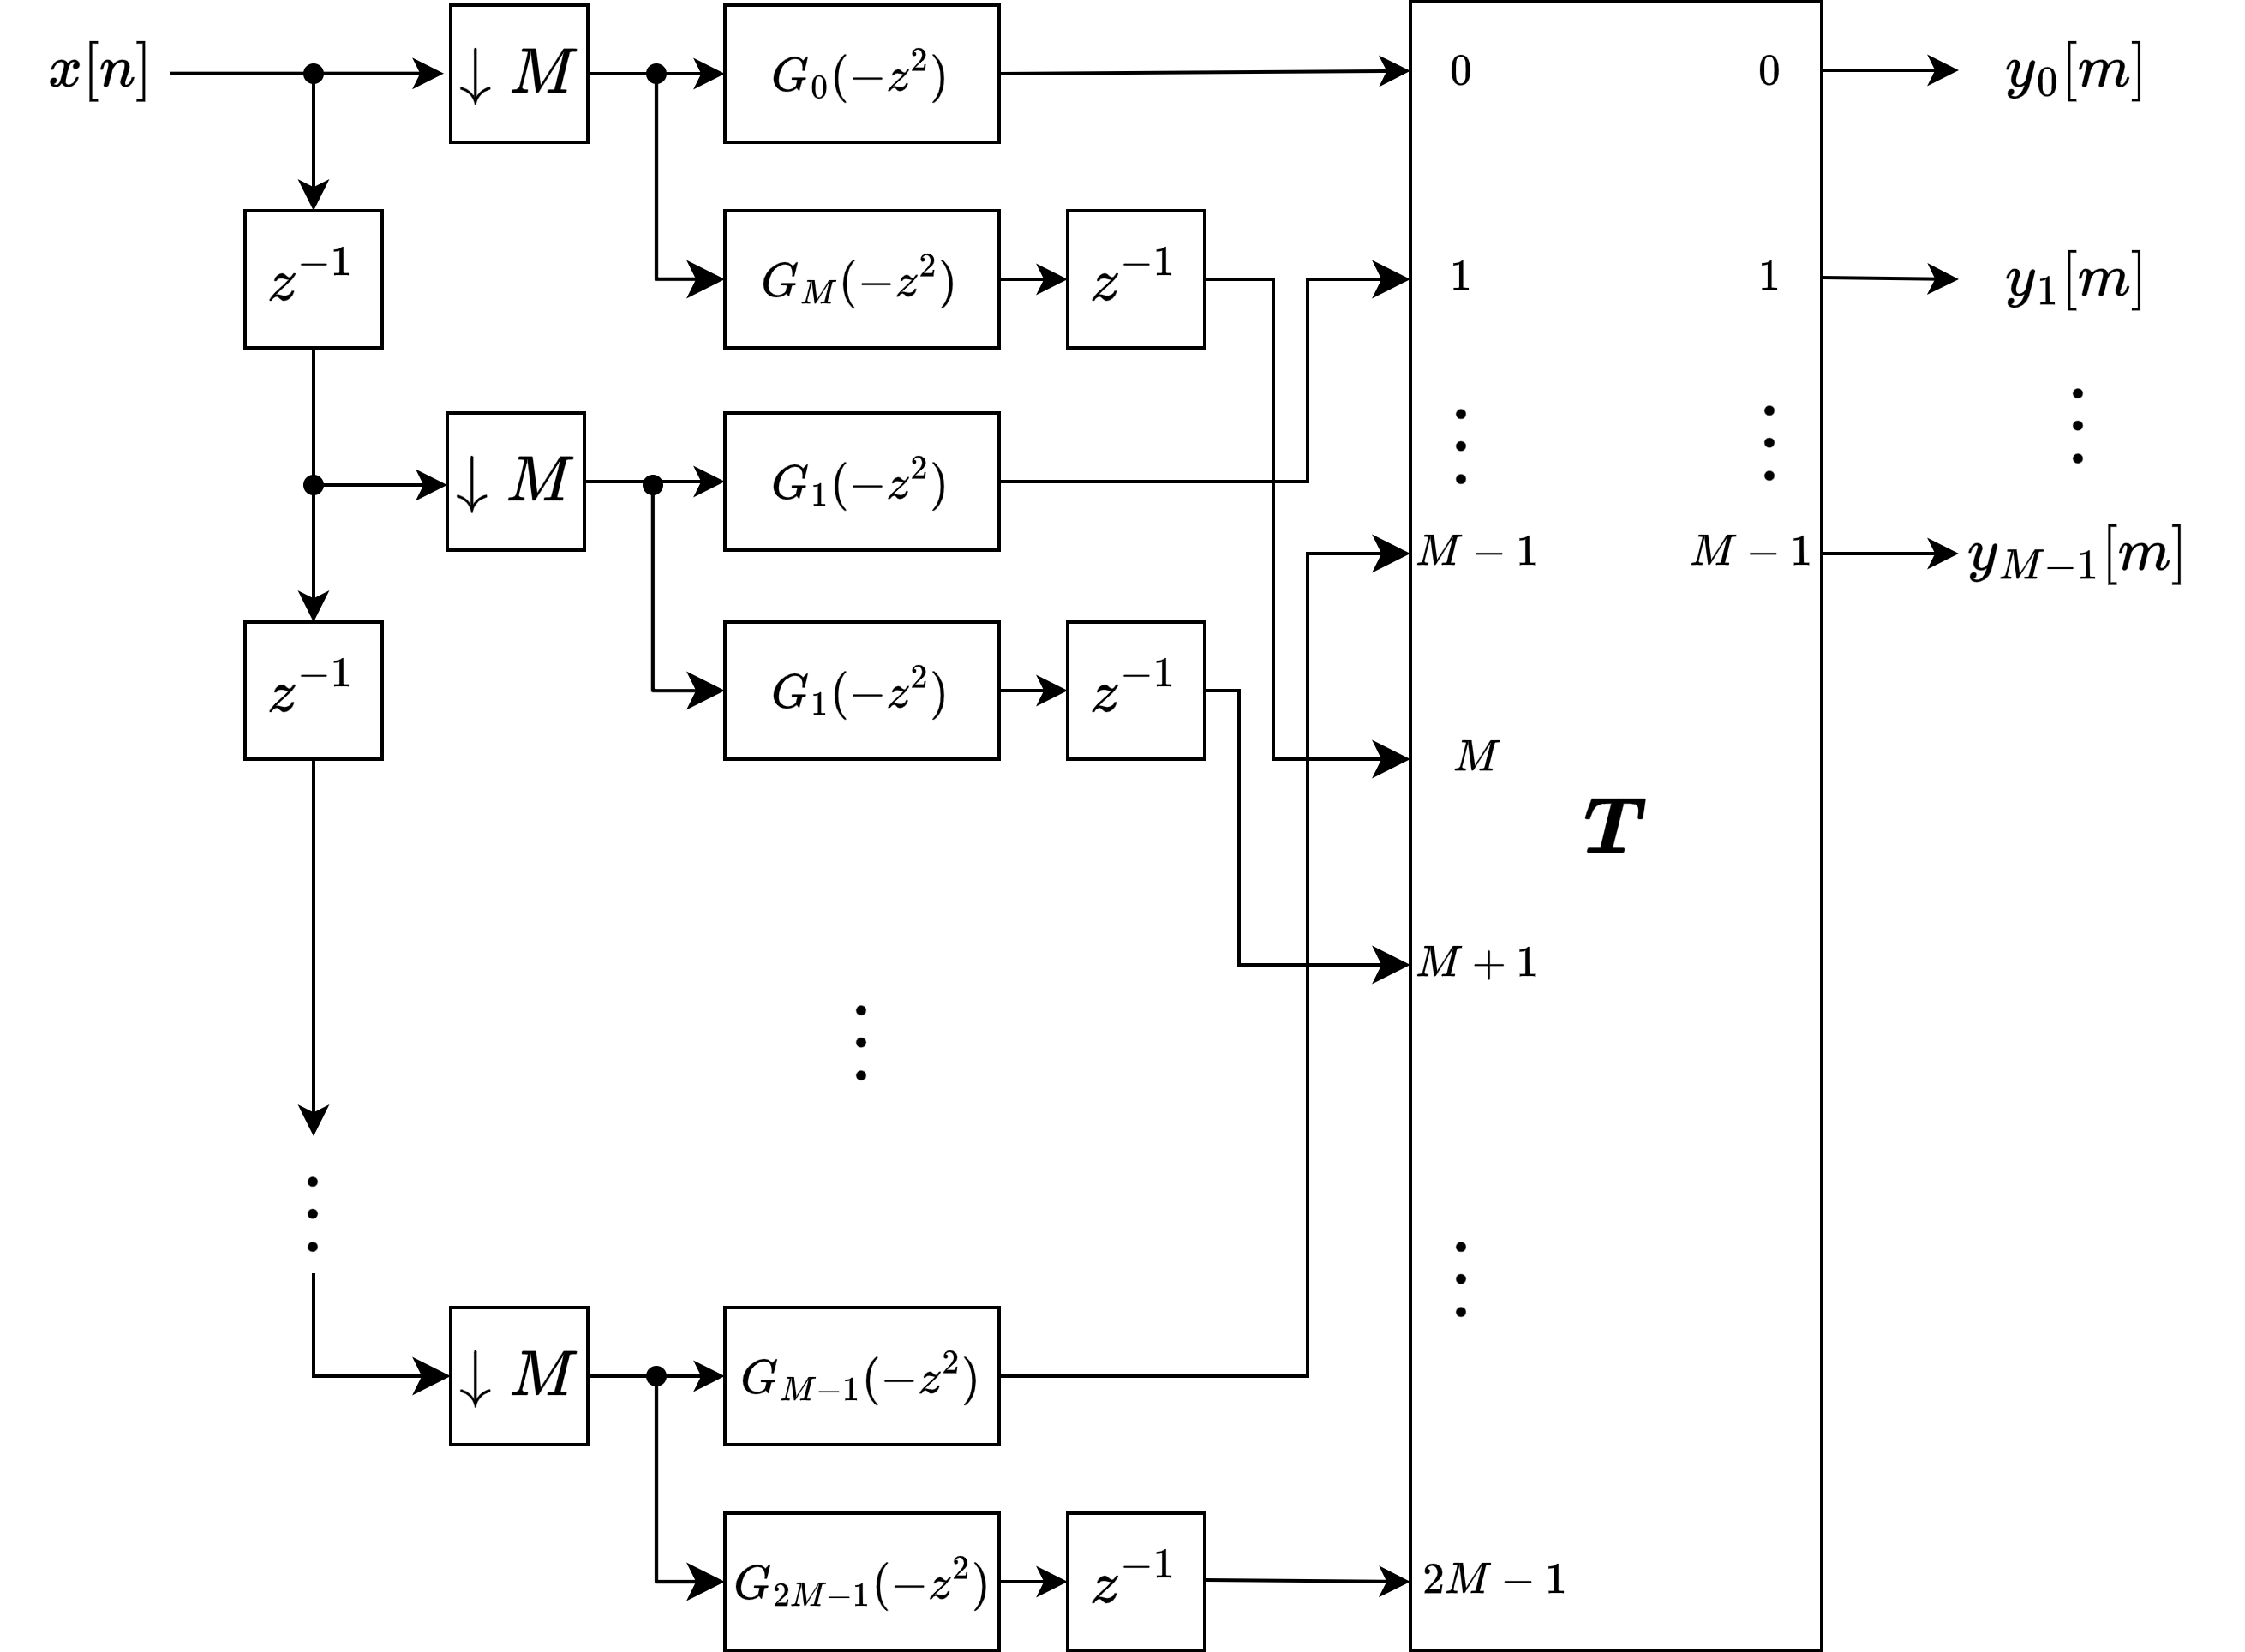
\includegraphics[width=95mm]{./figs/cos_modulated_analysis_bank_filter.drawio.png}
        \caption*{アナライザの構成}
    \end{figure}
\end{frame}

\begin{frame}[c]
    \frametitle{コサイン変調フィルタバンク}
    \begin{figure}
        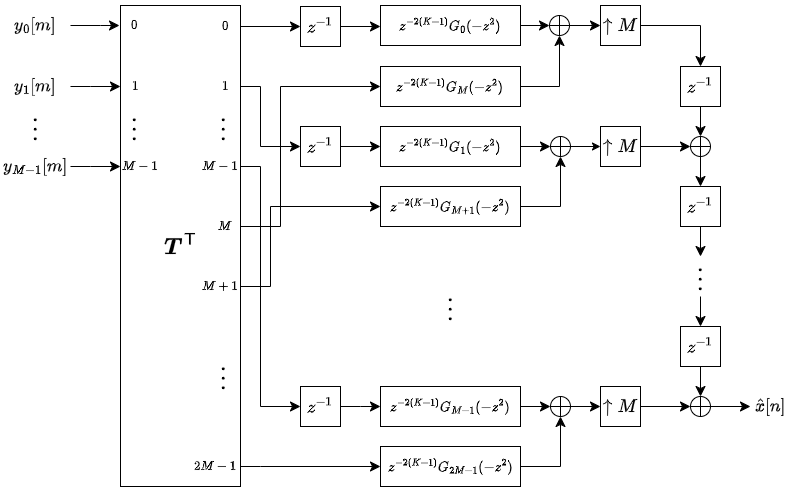
\includegraphics[width=115mm]{./figs/cos_modulated_synthesis_bank_filter.drawio.png}
        \caption*{シンセサイザの構成}
    \end{figure}
\end{frame}

\begin{frame}[c]
    \frametitle{コサイン変調フィルタバンク}
    完全再構成条件を導く.\eqref{eq:analyzer_matrix_of_cos_modulated_filter_bank},\eqref{eq:synthesizer_matrix_of_cos_modulated_filter_bank}式より,
    \begin{align*}
        & \ve{R}(z)\ve{E}(z) = z^{-(2K - 1)} \widetilde{\ve{E}}(z) \ve{E}(z) \\
        &= z^{-(2K - 1)} 
        \begin{bNiceMatrix}[margin, nullify-dots, xdots/shorten=0.5em]
            \ve{G}_{0}(z^{-1}) & z \ve{G}_{1}(z^{-1})
        \end{bNiceMatrix}
        \ve{T}^{\mathsf{T}} \ve{T}
        \begin{bNiceMatrix}[margin, nullify-dots, xdots/shorten=0.5em]
            \ve{G}_{0}(z) \\
            z^{-1} \ve{G}_{1}(z)
        \end{bNiceMatrix} \\
        &= 2M z^{-(2K - 1)} \left\{ \ve{G}_{0}(z^{-1}) \ve{G}_{0}(z) + \ve{G}_{1}(z^{-1}) \ve{G}_{1}(z) \right\}
    \end{align*}
    ここで,$\ve{T}^{\mathsf{T}} \ve{T} = 2M \ve{I}$(後で示す).$\ve{G}_{0}, \ve{G}_{1}$は対角行列だから,$k = 0, ..., M-1$に対し,
    \begin{align*}
        G_{k}(z^{-1}) G_{k}(z) + G_{M + k}(z^{-1}) G_{M + k}(z) = \alpha
    \end{align*}
    を満たせば完全再構成となる
\end{frame}

\begin{frame}[c]
    \frametitle{$\ve{T}^{\mathsf{T}} \ve{T} = 2M\ve{I}$の証明}
    $\left( \ve{T}^{\mathsf{T}} \ve{T} \right)_{ij} = \sum_{k = 0}^{M - 1} t_{k,i} t_{k,j}$であり,
    \scriptsize
    \begin{align*}
        & t_{k,i} t_{k,j} \\
        &= 4 \cos\left[ \frac{\pi}{M} \left( k + \frac{1}{2} \right) \left( i - \frac{L - 1}{2} \right) + (-1)^{k}\frac{\pi}{4} \right] \cos\left[ \frac{\pi}{M} \left( k + \frac{1}{2} \right) \left( j - \frac{L - 1}{2} \right) + (-1)^{k}\frac{\pi}{4} \right] \\
        &= 2 \left\{ \cos\left[ \frac{\pi}{M} \left( k + \frac{1}{2} \right) \left( i + j - \frac{L - 1}{2} \right) k + (-1)^{k} \frac{\pi}{2} \right] + \cos\left[ \frac{\pi}{M} \left( k + \frac{1}{2} \right) \left( i - j \right) \right] \right\}
    \end{align*}
    \normalsize
    $i + j - (L - 1) = A$とおくと,
    \scriptsize
    \begin{align*}
        & \cos\left[ \frac{\pi}{M} \left( k + \frac{1}{2} \right)A + (-1)^{k}\frac{\pi}{2} \right] \\
        &= \cos\left[ \frac{\pi}{M} \left( k + \frac{1}{2} \right)A \right] \cos\left[(-1)^{k}\frac{\pi}{2} \right] - \sin\left[ \frac{\pi}{M} \left( k + \frac{1}{2} \right)A \right] \sin\left[(-1)^{k}\frac{\pi}{2} \right] \\
        &= -(-1)^{k} \sin \left[ \frac{\pi}{M} \left( k + \frac{1}{2} \right)A \right]
    \end{align*}
\end{frame}

\begin{frame}[c]
    \frametitle{$\ve{T}^{\mathsf{T}} \ve{T} = 2M\ve{I}$の証明}
    ここで,
    \begin{align}
        \sum_{k = 0}^{M - 1}\cos\left[ \frac{\pi}{M} \left( k + \frac{1}{2} \right) \left( i - j \right) \right] &= M\delta_{ij} \label{eq:orthogonal_condition_cos} \\
        \sum_{k = 0}^{M - 1}(-1)^{k} \sin \left[ \frac{\pi}{M} \left( k + \frac{1}{2} \right)A \right] &= 0 \label{eq:orthogonal_condition_sin}
    \end{align}
    ($\delta_{ij}$:クロネッカーのデルタ)を示せば,
    \begin{align*}
        \left( \ve{T}^{\mathsf{T}} \ve{T} \right)_{ij} = 2M \delta_{ij}
    \end{align*}
    となり命題が示せる.次ページから計算結果を載せる
\end{frame}

\begin{frame}[c]
    \frametitle{$\ve{T}^{\mathsf{T}} \ve{T} = 2M\ve{I}$の証明}
    \eqref{eq:orthogonal_condition_cos}式を示す.$i = j$のとき,
    \scriptsize
    $\sum_{k = 0}^{M - 1} \cos\left[ \frac{\pi}{M} \left( k + \frac{1}{2} \right) ( i - j ) \right] = M$.
    \normalsize
    $i \neq j$のとき,
    \scriptsize
    \begin{align*}
        & \sum_{k = 0}^{M - 1} \cos\left[ \frac{\pi}{M} \left( k + \frac{1}{2} \right) ( i - j ) \right] \\
        &= \frac{1}{2} \sum_{k = 0}^{M - 1} \left\{ \exp\left[ j \frac{\pi}{M}  \left( k + \frac{1}{2} \right) (i - j) \right] + \exp\left[ -j \frac{\pi}{M} \left( k + \frac{1}{2} \right) (i - j) \right] \right\} \\
        &= \frac{1}{2} \sum_{k = 0}^{M - 1} \left\{ W_{2M}^{-\left( k + \frac{1}{2} \right)(i - j)} + W_{2M}^{\left( k + \frac{1}{2} \right)(i - j)} \right\} \nonumber \\
        &= \frac{1}{2} \left\{ W_{2M}^{-\frac{i - j}{2}} \sum_{k = 0}^{M - 1} W_{2M}^{-(i - j)k} + W_{2M}^{\frac{i - j}{2}} \sum_{k = 0}^{M - 1} W_{2M}^{(i - j)k} \right\} \\
        &= \frac{1}{2} \left[ \frac{W_{2M}^{-\frac{i - j}{2}}}{W_{2M}^{-(i - j)} - 1} \left\{ (-1)^{-(i - j)} - 1 \right\} + \frac{W_{2M}^{\frac{i - j}{2}}}{W_{2M}^{i - j} - 1} \left\{ (-1)^{i - j} - 1 \right\} \right]
    \end{align*}
    最後の式変形で等比級数の和$\sum_{k = 0}^{M - 1} W_{2M}^{(i - j)k} = \frac{W_{2M}^{(i -j)M} - 1}{W_{2M}^{i - j} - 1} = \frac{(-1)^{i - j} - 1}{W_{2M}^{i - j} - 1}$を使用
\end{frame}

\begin{frame}[c]
    \frametitle{$\ve{T}^{\mathsf{T}} \ve{T} = 2M\ve{I}$の証明}
    さらに式変形すると,
    \scriptsize
    \begin{align*}
        & \sum_{k = 0}^{M - 1} \cos\left[ \frac{\pi}{M} \left( k + \frac{1}{2} \right) ( i - j ) \right] \\
        &= \frac{1}{2} \left[ \frac{W_{2M}^{-\frac{i - j}{2}}}{W_{2M}^{-(i - j)} - 1} \left\{ (-1)^{-(i - j)} - 1 \right\} + \frac{W_{2M}^{\frac{i - j}{2}}}{W_{2M}^{i - j} - 1} \left\{ (-1)^{i - j} - 1 \right\} \right] \\
        &= \frac{W_{2M}^{-\frac{i - j}{2}} (W_{2M}^{i - j} - 1)\left\{ (-1)^{-(i - j)} - 1 \right\} + W_{2M}^{\frac{i - j}{2}} (W_{2M}^{-(i - j)} - 1)\left\{ (-1)^{i - j} - 1 \right\}}{2(W_{2M}^{-(i - j)} - 1)(W_{2M}^{i - j} - 1)} \\
        &= \frac{(W_{2M}^{\frac{i - j}{2}} - W_{2M}^{-\frac{i - j}{2}})\left\{ (-1)^{-(i - j)} - 1 \right\} + (W_{2M}^{-\frac{i - j}{2}} - W_{2M}^{\frac{i - j}{2}})\left\{ (-1)^{i - j} - 1 \right\}}{2(W_{2M}^{-(i - j)} - 1)(W_{2M}^{i - j} - 1)} \\
        &= \frac{(W_{2M}^{\frac{i - j}{2}} - W_{2M}^{-\frac{i - j}{2}})\left\{ (-1)^{i - j} - 1 \right\} + (W_{2M}^{-\frac{i - j}{2}} - W_{2M}^{\frac{i - j}{2}})\left\{ (-1)^{i - j} - 1 \right\}}{2(W_{2M}^{-(i - j)} - 1)(W_{2M}^{i - j} - 1)} \\
        &= 0
    \end{align*}
    \normalsize
    よって\eqref{eq:orthogonal_condition_cos}式が示された
\end{frame}

\begin{frame}[c]
    \frametitle{$\ve{T}^{\mathsf{T}} \ve{T} = 2M\ve{I}$の証明}
    \eqref{eq:orthogonal_condition_sin}式を示す.
    \scriptsize
    \begin{align*}
        & \sum_{k = 0}^{M - 1} (-1)^{k} \sin\left[ \frac{\pi}{M} \left( k + \frac{1}{2} \right) A  \right] \\
        &= \frac{1}{j2} \sum_{k = 0}^{M - 1} (-1)^{k} \left\{ \exp\left[ j \frac{\pi}{M} \left( k + \frac{1}{2} \right) A  \right] - \exp\left[ -j \frac{\pi}{M} \left( k + \frac{1}{2} \right) A  \right] \right\} \\
        &= \frac{1}{j2} \sum_{k = 0}^{M - 1} (-1)^{k} \left\{ W_{2M}^{-A\left( k + \frac{1}{2} \right)} - W_{2M}^{A\left( k + \frac{1}{2} \right)} \right\} \\
        &= \frac{1}{j2} \left\{ W_{2M}^{-\frac{A}{2}} \sum_{k = 0}^{M - 1} (-1)^{k} W_{2M}^{-Ak} - W_{2M}^{\frac{A}{2}} \sum_{k = 0}^{M - 1} (-1)^{k} W_{2M}^{Ak} \right\} \\
        &= \frac{1}{j2} \left\{ W_{2M}^{-\frac{A}{2}} \sum_{k = 0}^{M - 1} W_{2M}^{-(M + A)k} - W_{2M}^{\frac{A}{2}} \sum_{k = 0}^{M - 1} W_{2M}^{(M + A)k} \right\} \quad \text{($\because$ $(-1)^{k} = W_{2M}^{M} = W_{2M}^{-M}$)} \\
        &= \frac{1}{j2} \left\{ W_{2M}^{-\frac{A}{2}} \frac{(-1)^{-(M + A)} - 1}{W_{2M}^{-(M + A)} - 1} - W_{2M}^{\frac{A}{2}} \frac{(-1)^{M + A} - 1}{W_{2M}^{M + A} - 1} \right\} \quad \text{($\because$ 等比級数の和の公式)}
    \end{align*}
\end{frame}

\begin{frame}[c]
    \frametitle{$\ve{T}^{\mathsf{T}} \ve{T} = 2M\ve{I}$の証明}
    さらに計算を進めると,
    \scriptsize
    \begin{align*}
        & \sum_{k = 0}^{M - 1} (-1)^{k} \sin\left[ \frac{\pi}{M} \left( k + \frac{1}{2} \right) A \right] \\
        &= \frac{W_{2M}^{-\frac{A}{2}} \left\{ (-1)^{-(M + A)} - 1 \right\} (W_{2M}^{M + A} - 1) - W_{2M}^{\frac{A}{2}} \left\{ (-1)^{M + A} - 1 \right\} (W_{2M}^{-(M + A)} - 1)}{j2(W_{2M}^{-(M + A)} - 1)(W_{2M}^{(M + A)} - 1)} \\
        &= \frac{(-1)^{-(M + A)} W_{2M}^{M + \frac{A}{2}} - W_{2M}^{M + \frac{A}{2}} - (-1)^{M + A} W_{2M}^{-M - \frac{A}{2}} + W_{2M}^{-M - \frac{A}{2}}}{j2(W_{2M}^{-(M + A)} - 1)(W_{2M}^{(M + A)} - 1)} \\
        &= \frac{(-1)^{A}(W_{2M}^{-\frac{A}{2}} - W_{2M}^{\frac{A}{2}}) - (-1)(W_{2M}^{-\frac{A}{2}} - W_{2M}^{\frac{A}{2}})}{j2(W_{2M}^{-(M + A)} - 1)(W_{2M}^{(M + A)} - 1)} \\
        &= \frac{-j2 (-1)^{A} \sin\left( \frac{\pi A}{2M} \right) -j2  \sin\left( \frac{\pi A}{2M} \right)}{j2(W_{2M}^{-(M + A)} - 1)(W_{2M}^{(M + A)} - 1)} = -\frac{\sin\left( \frac{\pi A}{2M} \right) \left\{ (-1)^{A} + 1 \right\}}{j2(W_{2M}^{-(M + A)} - 1)(W_{2M}^{(M + A)} - 1)}
    \end{align*}
    \normalsize
    最後の式の分子は,$A$の偶奇に関わらず$0$.よって,\eqref{eq:orthogonal_condition_sin}式が示された.
\end{frame}

\begin{frame}[c]
    \frametitle{MP3のフィルタバンクの特性}
    \vspace{-5pt}
    \begin{figure}
        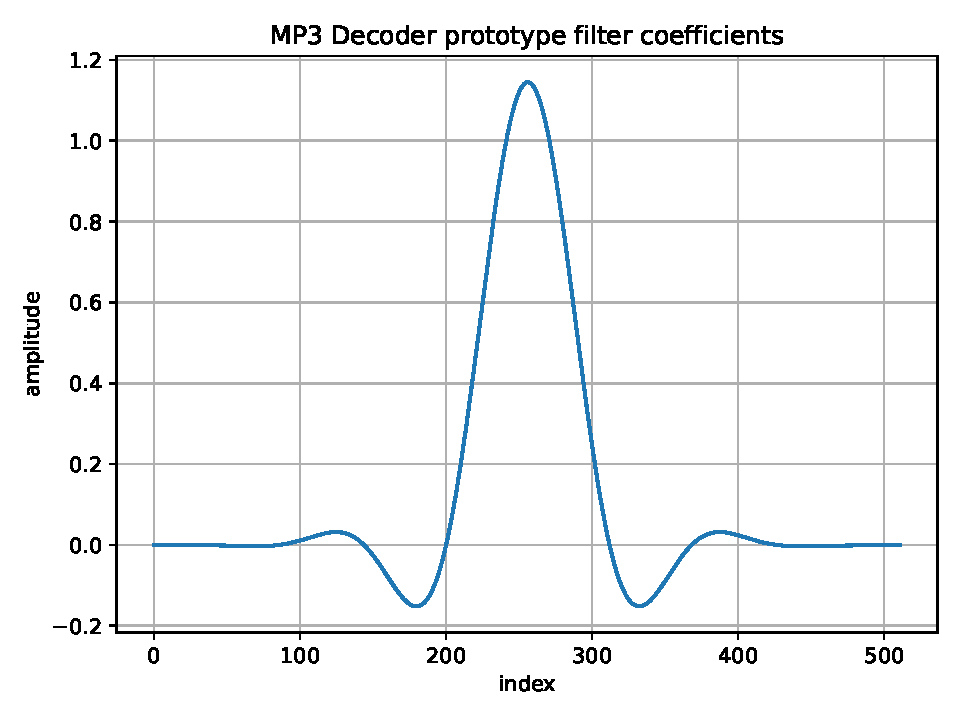
\includegraphics[width=100mm]{./figs/mp3_decoder_prototype_filter_coef.pdf}
    \end{figure}
    \vspace{-5pt}
    \begin{itemize}
        \item デコーダの係数.エンコーダの係数の$32$倍
    \end{itemize}
\end{frame}

\end{document}
